% \date{May 14, 2024}
% \author{Deralive / Shichien}
% \title{华东师范大学软件学院实验报告模板}
% 注意事项:编译两次,以确保目录、页码完整显示
% 模板文件:https://github.com/Shichien/ECNU-LateX-Template

\def\allfiles{}

\documentclass[14pt,a4paper,UTF8,twoside]{article}

\usepackage{amsmath}
\usepackage{graphicx}
\usepackage{longtable}
\usepackage{geometry} 
\usepackage{ctex}
\usepackage{booktabs} % 表格库
\usepackage{titlesec} % 标题库
\usepackage{fancyhdr} % 页眉页脚库
\usepackage{lastpage} % 页码数库
\usepackage{listings} % 代码块包
\usepackage{xcolor}
\usepackage[hidelinks]{hyperref}
\usepackage{tikz}
\usepackage{tikz-qtree}
\usepackage{fontspec} % 允许设置字体
\usepackage{unicode-math} % 允许数学公式使用特定字体
\usepackage{mwe}
\usepackage{zhlipsum} % 中文乱数文本
\usepackage{amsmath}
\usepackage{xcolor}
\usepackage{float} % 浮动体环境
\usepackage{subcaption} % 子图包
\usepackage{biblatex}
\usepackage{forest}
\addbibresource{references.bib} % 指定你的.bib文件名称

\definecolor{mygreen}{rgb}{0,0.6,0}
\definecolor{mygray}{rgb}{0.5,0.5,0.5}
\definecolor{mymauve}{rgb}{0.58,0,0.82}

\date{} % 留空,以让编译时去除日期

%———————————————注意事项—————————————————%

% 1、如果编译显示失败,但没有错误信息,就是 filename.pdf 正在被占用
% 2、在文件夹中的终端使用 Windows > xelatex filename.tex 也可编译

%—————————————华东师范大学———————————————%

% 论文制作时须加页眉,页眉从中文摘要开始至论文末
% 偶数页码内容为:华东师范大学硕士学位论文,奇数页码内容为学位论文题目

%————————定义 \section 的标题样式————————%

% 注意:\chapter 等命令,内部使用的是 \thispagestyle{plain} 的排版格式
% 若需要自己加上页眉,实际是在用 \thispagestyle{fancy} 的排版格式
% 加上下面这一段指令,就能够让 \section 也使用 fancy 的排版格式
% 本质就是让目录、第一页也能够显示页眉、页脚

\fancypagestyle{plain}{
  \pagestyle{fancy}
}

\title{华东师范大学软件学院课程项目报告} % 模板
\titleformat{\section}
    {\normalfont\bfseries\Large} % 字体大小、字体系列(\bfseries 为加粗)
    {\thesection}{1em}{}

% 设置章节的中文格式
\renewcommand\thesection{\chinese{section} \hspace{0pt}}
\renewcommand\thesubsection{\arabic{subsection} \hspace{0pt}}
% \renewcommand\thesubsubsection{\alph{subsubsection} \hspace{0pt}} % 字母编号
% \hspace{0pt} 是为了确保在章节编号和章节题目之间不要有空格,使得排版更为美观
    
%—————————————页面基础设置———————————————%

\geometry{left=10mm, right=10mm, top=20mm, bottom=20mm}

%————————————设置页眉、页脚——————————————%

\pagestyle{fancy} % 设置 plain style 的属性

% 设置页眉
% 使用 \footnotesize 确保章节名和标题名不会重合(缩小字体)

\fancyhead[RE]{\footnotesize \leftmark} % Right Even 偶数页右侧显示章名 \leftmark 最高级别章名
\fancyhead[LO]{\footnotesize \rightmark} % Left Odd 奇数页左侧显示节名 \rightmark 第二级别节名
\fancyhead[C]{华东师范大学软件学院课程项目报告} % Center 居中显示
\fancyhead[LE,RO]{~\thepage~} % 在偶数页的左侧,奇数页的右侧显示页码
\renewcommand{\headrulewidth}{1.2pt} % 页眉与正文之间的水平线粗细

% 设置页脚:在每页的右下脚以斜体显示书名

\fancyfoot[RO,RE]{\it Lab Report By \LaTeX} % 使用意大利斜体显示
\renewcommand{\footrulewidth}{0.5pt} % 页脚水平线宽度

% 设置页码:在底部居中显示页码

\pagestyle{fancy}
\fancyfoot[C]{\kaishu 第 \thepage 页 \ 共 \pageref{LastPage} 页} % LastPage 需要二次编译以获取总页数

%——————————————代码块设置———————————————%

\lstset {
    backgroundcolor=\color{white},   % choose the background color; you must add \usepackage{color} or \usepackage{xcolor}
    basicstyle=\footnotesize,        % the size of the fonts that are used for the code
    breakatwhitespace=false,         % sets if automatic breaks should only happen at whitespace
    breaklines=true,                 % sets automatic line breaking
    captionpos=bl,                   % sets the caption-position to bottom
    commentstyle=\color{mygreen},    % comment style
    deletekeywords={...},            % if you want to delete keywords from the given language
    escapeinside={\%*}{*},           % if you want to add LaTeX within your code
    extendedchars=true,              % lets you use non-ASCII characters; for 8-bits encodings only, does not work with UTF-8
    frame=single,                    % adds a frame around the code
    keepspaces=true,                 % keeps spaces in text, useful for keeping indentation of code (possibly needs columns=flexible)
    keywordstyle=\color{blue},       % keyword style
    % language=Python,               % the language of the code
    morekeywords={*,...},            % if you want to add more keywords to the set
    numbers=left,                    % where to put the line-numbers; possible values are (none, left, right)
    numbersep=5pt,                   % how far the line-numbers are from the code
    numberstyle=\tiny\color{mygray}, % the style that is used for the line-numbers
    rulecolor=\color{black},         % if not set, the frame-color may be changed on line-breaks within not-black text (e.g. comments (green here))
    showspaces=false,                % show spaces everywhere adding particular underscores; it overrides 'showstringspaces'
    showstringspaces=false,          % underline spaces within strings only
    showtabs=false,                  % show tabs within strings adding particular underscores
    stepnumber=1,                    % the step between two line-numbers. If it's 1, each line will be numbered
    stringstyle=\color{orange},      % string literal style
    tabsize=2,                       % sets default tabsize to 2 spaces
    % title=Python Code              % show the filename of files included with \lstinputlisting; also try caption instead of title
}

% 注释掉的部分用于后续插入代码,参数可调整,格式如下:

% 1、直接插入
% \begin{lstlisting}[language = ? , title = { ? } ]
%       Your code here.
% \end{lstlisting}

% 2、文件插入
% \lstinputlisting[language = C , title = ?.c] {filename.c}

%———————————————字体设置————————————————%

% \setCJKmainfont{SimSun} % 设置正文罗马族的 CJK 字体
% \renewcommand{\normalsize}{\fontsize{12pt}{15pt}\selectfont} % 设置正文字号
\linespread{1.2}

%———————————————超链接设置——————————————%

\hypersetup{
    pdfstartview=FitH, % 设置PDF文档打开时的初始视图为页面宽度适应窗口宽度(即页面水平适应)
    CJKbookmarks=true, % 用对CJK(中文、日文、韩文)字符的书签支持,确保这些字符在书签中正确显示
    bookmarksnumbered=true, % 书签带有章节编号。这对有章节编号的文档很有用
    bookmarksopen=true, % 文档打开时,书签树是展开的,方便查看所有书签
    colorlinks, % 启用彩色链接。这样,链接在PDF中会显示为彩色,而不是默认的方框
    pdfborder=001, % 设置PDF文档中链接的边框样式。001 表示链接周围没有边框,仅在单击时显示一个矩形
    linkcolor=blue, % 设置文档内部链接(如目录中的章节链接)的颜色为蓝色
    anchorcolor=blue, % 设置锚点链接(即目标在同一文档内的链接)的颜色为蓝色
    citecolor=blue, % 设置引用(如文献引用)的颜色为蓝色
}

%——————————————导言区结束,进入正文部分———————————————%

%——————————————————————————————————————%

\begin{document}

\maketitle

\begin{center} % \extracolsep{\fill} 拉伸到页面最大宽度前,保证居中显示

    \begin{tabular*}{\textwidth}{@{\extracolsep{\fill}} l  l  l }
        \hline
        课程名称:创客实践 & 成绩:\\
        姓名:张梓卫 & 学号:10235101526\\
        指导老师:陈闻杰 & 日期:2024/8/10\\
        项目名称:基于LLM的\textit{ESP32}智能设备多功能控制系统 & 班级:软工3班\\
        \hline
    \end{tabular*}

\end{center}

\tableofcontents % 目录也需要二次编译

%————————————————————————————————————————————————————————————

\section{项目简介}


\subsection{项目介绍}

本项目以 ESP32 为主控,使用 LLM(讯飞星火大模型)运行语音识别与在线联网回答。
基于 MQTT、HTTP、ESP-NOW 协议实现远程云端传输、近程数据传输。
通过外接传感器实现动态数据读取,在线数据反馈,实现了基于物联网的智能外接设备控制系统。

课程项目源代码及相关文件链接:\href{https://github.com/Shichien/Maker-practice}{\underline{https://github.com/Shichien/Maker-practice}}

\subsection{项目主要功能及应用场景}

本项目通过多种传感器测量室内示数:如$CH_4、H_2、CH_3COOH、LPG、温度、湿度$等,
实时通过 MQTT 协议传输至云端,在各地均可通过微信小程序或 OneNET 平台调试器进行远程读数,获取室内情况,以及远程控制室内各模块。
项目同时实现全智能无线连接,通过语音识别判断用户需求,实时语音播报室内信息;连接大模型,模块可联网实现提问与回答。

通过 ESP-NOW 协议绕过 WiFi ,实现伪 AC + AP 组网模式,多接入点可实现任意规模大小接入,通过 ESP-NOW 协议实现短距离无线通信,
可以连接任意接口进行函数调用输出。

火焰传感器与光照传感器、雨滴传感器可实时监控室内的特殊天气、事件情况,传输给云端进行数据处理,报警等操作。

\subsection{硬件物料}

\begin{itemize}
    \item ESP-WROOM-32 开发板、ESP-8266-Mod 开发板
    \item 1.8 寸 RGB-TFT OLED、SSD 1306 OLED
    \item INMP441 MEMS 麦克风
    \item MAX98357 I2S 音频放大器
    \item LB 喇叭
    \item DHT22、MPU6050、LM393、MQ5、MQ135 传感器
    \item MH-RD Raindrops Module
    \item 无刷电机(Fan Module)
\end{itemize}

    具体的接线图及引脚定义图请见【\textcolor{mygreen}{附件}】

\subsection{To Do List}

\begin{itemize}
    \item 上传时删除库文件中的 Sample 例子
    \item 使用 Ollama 部署本地推断模型与 ESP32 交汇
    \item 基于阿里云进行 MQTT 协议通信以及远程控制、点灯等操作
    \item 在 PlatformIO 平台上有一个库是 Aliyun IOT SDK,注意后续可能要用到
    \item 使用 MPU6050 进行云台自控制
\end{itemize}

\subsection{项目环境及工具列表}

本项目设计的环境为 Windows 11,开发板编程使用 Clion Platform,
选择 Upesy\_Wroom 开发环境,Arduino 框架,模拟仿真平台使用 Wokwi Simulator,
串口监视器选用 VOFA+ 1.3.10,波特率为115200(8N1),代码使用 Vim 编写,
课程报告使用 \LaTeX 撰写,并使用Git进行版本管理。

% —————————————————————————————————————————————————————————————

\section{技术原理}

\subsection{ESP32的使用及其硬件接口}

\begin{itemize}
    \item Espressif 32ESP32 集成了 2.4 GHz Wi-Fi 和 Bluetooth 4.2 LE(低功耗)功能,使其能够在无线网络环境中轻松实现连接和数据传输。
    \item 提供了丰富的外设接口,包括多达 34 个 GPIO 引脚、ADC(模数转换器)、DAC(数模转换器)、SPI、I2C、UART、PWM、CAN 总线。
\end{itemize}

\subsection{基于LLM、TTS语音识别与合成}

随着 LLM 在近年来在世界各地火热传播,一位机器学习工程师与我说:“现在市场上是个软件就得说自己用了 AI,不然不好意思提供服务了”,此句稍带滑稽的话语让我萌生了使用LLM的念头。
灵活高效、易于使用。在本项目中,主要用于流式语音识别及语音生成转换(基于讯飞的星火大模型Spark Ultra 4.0)。

\subsection{FreeRTOS、Ticker多任务调度}

FreeRTOS 是一个广泛用于嵌入式开发的实时操作系统,提供多任务调度、任务间通信、优先级管理等功能,
vTaskDelay() 是 FreeRTOS 提供的任务延迟函数,用于让当前任务进入阻塞状态,释放 CPU 给其他任务使用。
ESP32已经包含了FreeROTS内核,使用 vTaskDelay,可以避免Delay()函数造成的整体阻塞。

同时,Ticker计时器可以使用一行代码实现多任务调度的管理:\texttt{ticker.attach(Time,FunctionName);}

\subsection{基于HTTP、ESP-NOW通信协议的使用}

ESP-NOW 是一种轻量级、低功耗的点对点(P2P)通信协议,专为短距离设备之间的快速数据传输而设计。
不依赖于传统的 Wi-Fi 网络和路由器。
ESP-NOW 允许多个设备(资料显示,最多20个,不然会超过ESP32的功耗)直接进行无线数据传输,适用于需要快速和实时通信的物联网应用场景。

HTTP 在客户端与服务器之间传输超文本数据,是互联网通信的基础,HTTPClient库提供各种接口,包括GET、POST请求,可以连接服务器后返回响应:
HTML、JSON数据等,使用ESP32可以远程连接各种API获取数据,如使用\underline{www.baidu.com} 获取 RFC1123 时间戳。

\subsection{基于MQTT物联网通信协议的使用}

MQTT 是一个轻量级的发布/订阅消息传输协议,广泛用于物联网设备之间的数据通信。
提供在不稳定网络环境中的低带宽、高延迟或间歇性连接情况下的可靠通信。
客户端可以是任何设备或应用程序(如传感器、服务器、移动设备),
它们可以作为发布者,也可以作为订阅者接收消息。

OneNET 是中国移动开发的物联网(IoT)开放平台,支持多种主流通信协议,如MQTT、HTTP、CoAP等,在此我使用MQTT协议进行传感器的上传。

\subsection{多种传感器综合实践}

Adafruit开源硬件公司各常用模块以及MH-Sensor系列是一系列传感器产品,包括温度传感器、湿度传感器、气压传感器
光照传感器等。这些传感器可以用于测量环境参数,例如温度、湿度、气压、光照等。

\subsubsection{MPU6050 六轴传感器}

MPU6050 集成了三轴加速度计和三轴陀螺仪,能够测量 X、Y、Z 三个方向上的加速度和角速度。
加速度计的测量范围为 ±2g、±4g、±8g 和 ±16g。
陀螺仪的测量范围为 ±250°/s、±500°/s、±1000°/s 和 ±2000°/s。
采用IIC总线接口通信。

\subsubsection{DHT22 湿温度传感器}

温度测量范围: -40°C 到 80°C,精度为 ±0.5°C。
湿度测量范围: 0\% 到 100\% 相对湿度,精度为 ±2\% RH。

DHT22 使用单线数字信号输出,易于与微控制器进行接口通信。

\subsubsection{LM393光照传感器}

LM393 的工作原理基于电压比较。
当正输入电压高于负输入电压时,输出为低电平(接近 0V)。
当正输入电压低于负输入电压时,输出为高电平(受上拉电阻决定),内置光敏电阻,可提供模拟信号。

\subsubsection{MQ系列气体传感器}

MQ传感器内部通常由一个加热元件和一个氧化锡(SnO2)半导体组成。当特定气体通过传感器时,氧化锡半导体的电导率会发生变化,这种变化可以被检测并转化为气体浓度。
每种MQ传感器的灵敏度曲线不同,对某些气体更敏感。例如,MQ-2对甲烷、丙烷和烟雾敏感,而MQ-7对一氧化碳更敏感。

注意:\textbf{MQ系列传感器一次只能检测一种气体的浓度值,但对于不同的气体分子,拥有不同的指数函数曲线,在定义不同的A、B值时读取}

\subsubsection{火焰传感器}

火焰传感器可以用来探测火源或其它波长在760纳米~1100纳米范围内的光源。
探测角度达60度,对火焰光谱特别灵敏。
注意,手机手电筒中也含有对应波长的光源。

\section{实现方法及步骤}

\subsection{基于LLM的语音识别与TTS语音合成}

要想在数字音频设备之间进行通信,可以使用I2S同步串行通信协议。

在ESP32中,有实现I2S协议的库:\href{https://github.com/schreibfaul1/ESP32-audioI2S}{\underline{https://github.com/schreibfaul1/ESP32-audioI2S}}

首先要进行语音识别的实现,我选择使用INMP441 MEMS全向麦克风进行实时录音。
接下来聚焦的痛点是:如何将录音数据传输到LLM中进行语音识别?

幸运的是,讯飞开放平台中提供了流式语音识别的API,可以将录音数据实时传输到LLM中进行语音识别。
\textbf{以下,我们将语音转文字(Speech To Text)简写为STT,文字转语音(Text To Speech)简写为TTS}。
下一步即调用API接口,进入官方文档中获取相关的参数。

\begin{figure} [H]
    \centering
    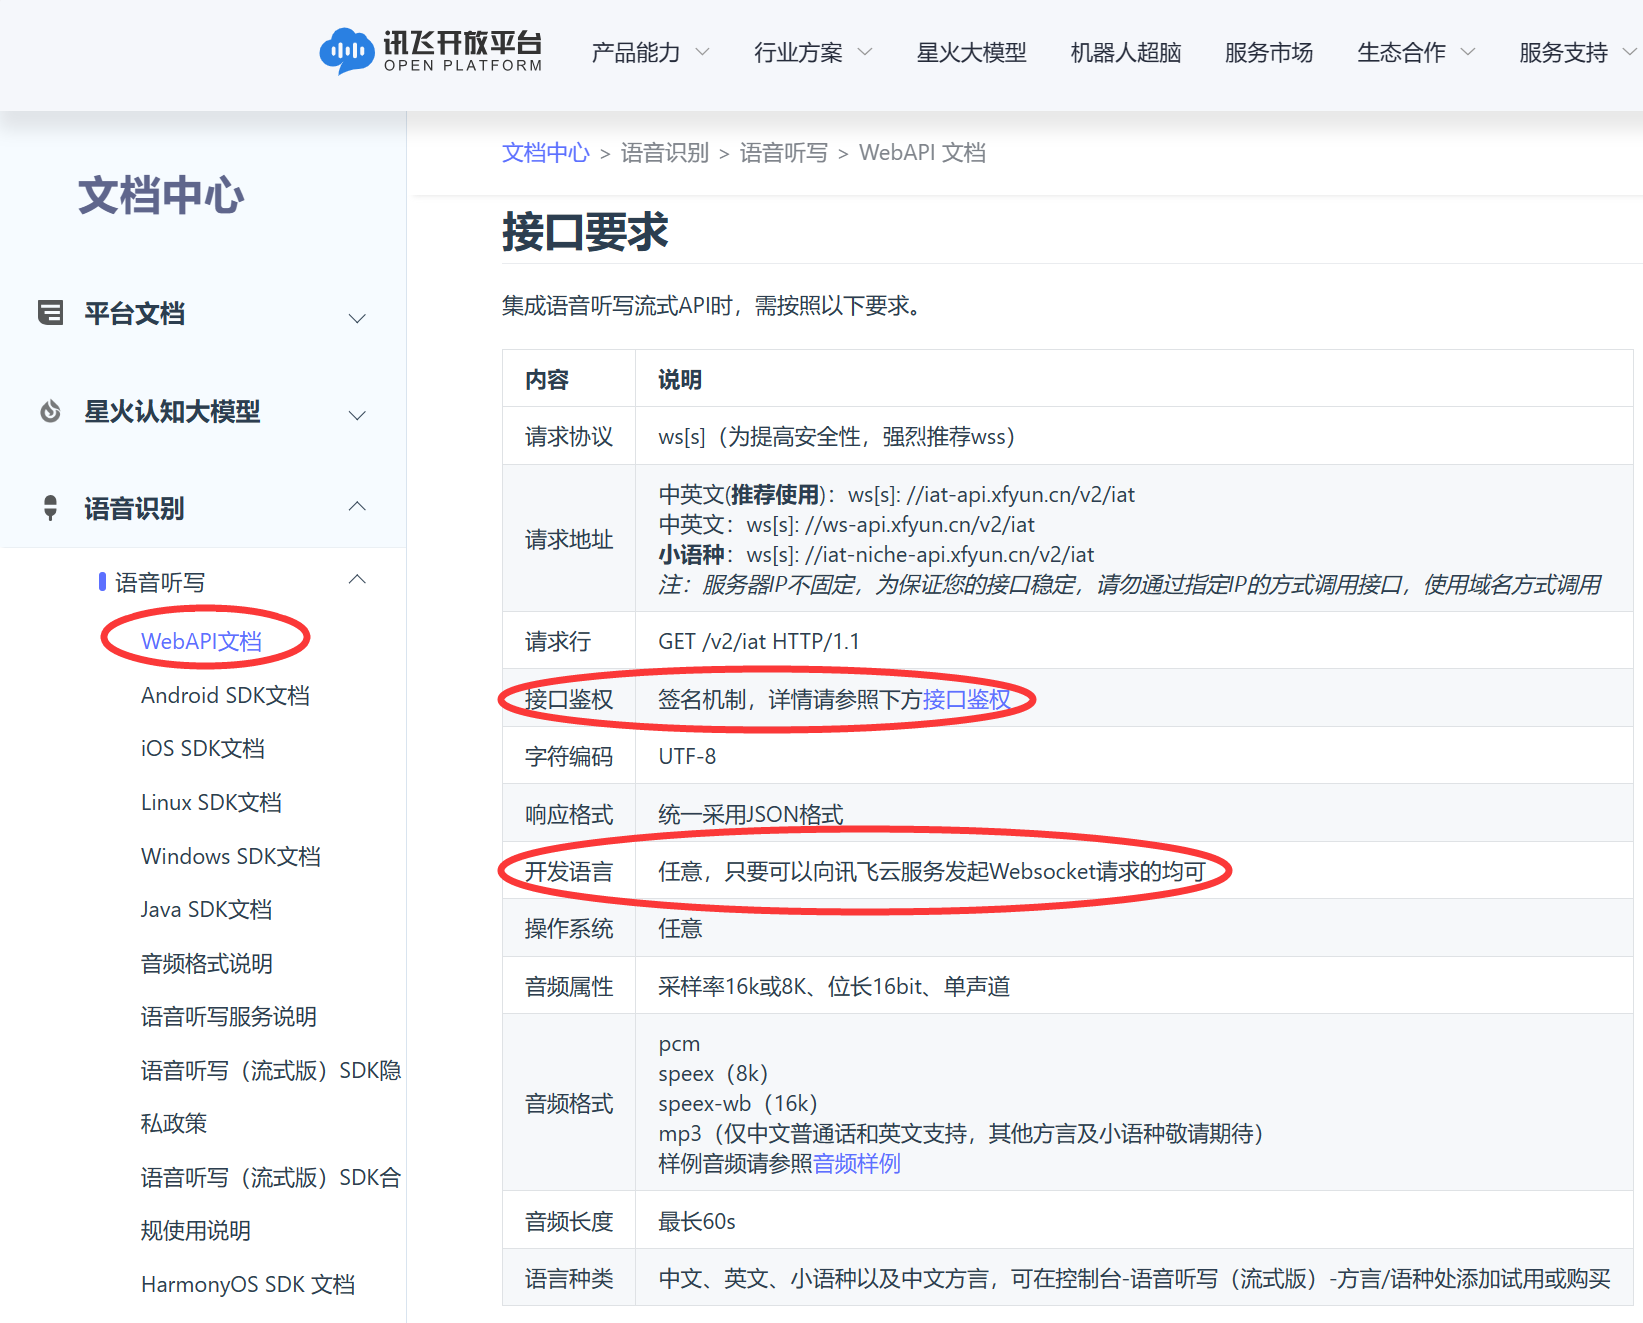
\includegraphics[width=0.53\textwidth]{../img/STTAPI.png}
    \caption{STT API接口参数列表}
    \label{fig:STTAPI}
\end{figure}

在调用接口时,需要按照下方所示的Url鉴权方法进行请求地址加鉴权参数的形式鉴权。

\begin{figure} [H]
    \centering
    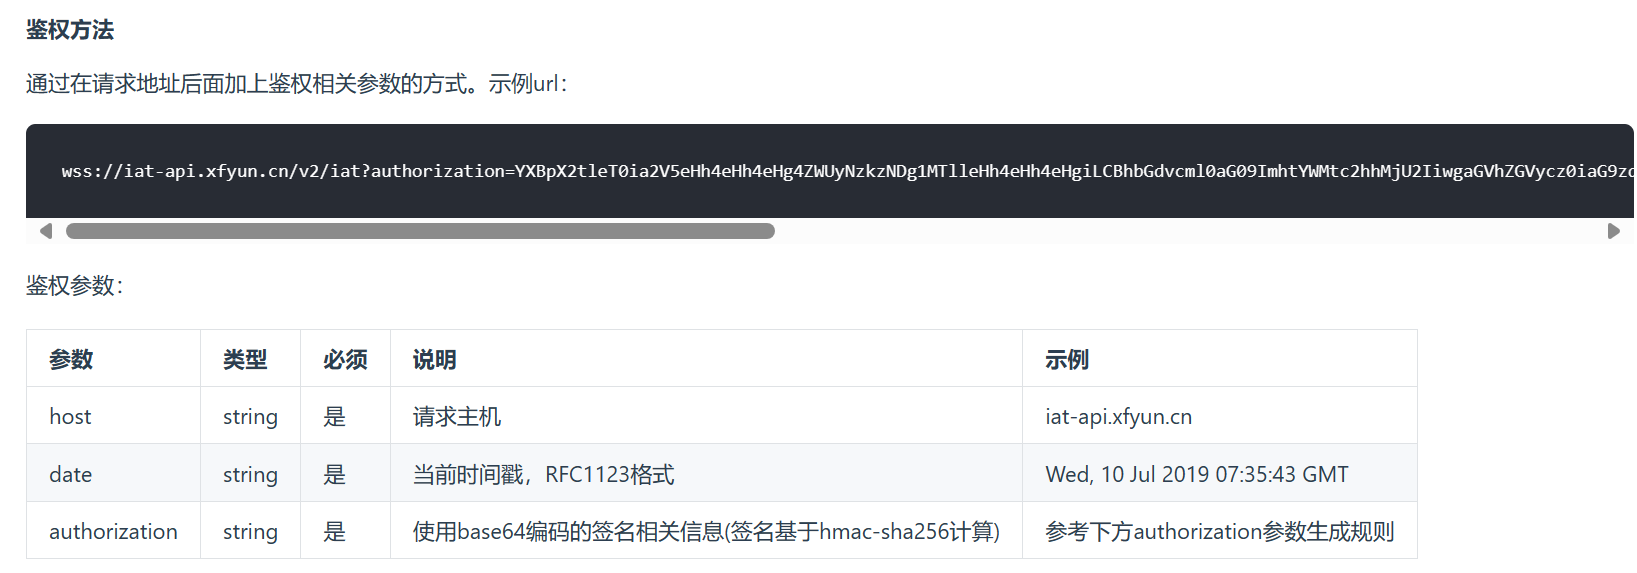
\includegraphics[width=0.6\textwidth]{../img/GetUrl.png}
    \caption{Url鉴权方法}
    \label{fig:Url Authorization}
\end{figure}

以下分别按照步骤进行鉴权:

\subsubsection{通过HTTP请求返回RFC 1123格式的时间戳}

\begin{lstlisting}[language = C++, title = {通过HTTP请求返回RFC1123格式的时间戳}]
void getRFC1123Time() {
    HTTPClient http;
    http.begin("https://www.baidu.com");

    // 从 HTTP 响应头中获取Date
    const char *headerKeys[] = {"Date"};
    http.collectHeaders(headerKeys, sizeof(headerKeys) / sizeof(headerKeys[0]));
    int httpCode = http.GET() ; // 必须要先设置收集字段,再发送HTTP请求,否则收集不到
    Date = http.header("Date");
    http.end();

    // Debug
    Serial.println("Date:" + Date);
    Serial.println("httpCode:" + httpCode);
}
\end{lstlisting}

\subsubsection{通过Hmac-sha256算法生成鉴权参数}

Hmac-sha256算法介绍部分见附件。此处我使用mbedTLS开源加密库实现算法。

\begin{lstlisting} [language = C++, title = {通过Hmac-sha256算法生成鉴权参数}]
String getOriginalSignature(String host, String date, String path) {
    return "host: " + host + "\n" + "date: " + date + "\n" + "GET " + path + " HTTP/1.1";
}

String getUrl(String Spark_url, String host, String path, String date) {
    String originalSignature = getOriginalSignature(host, date, path);
    const size_t originalSignatureLength = originalSignature.length(); // 原始签名的长度
    const size_t APIKeyLength = APISecret.length(); // API Key 的长度
    // 使用 HMAC-SHA256 进行加密
    unsigned char hmac[32]; // 存储HMAC结果
    mbedtls_md_context_t ctx; // HMAC上下文
    mbedtls_md_type_t md_type = MBEDTLS_MD_SHA256;
    mbedtls_md_init(&ctx);
    mbedtls_md_setup(&ctx, mbedtls_md_info_from_type(md_type), 1);
    mbedtls_md_hmac_starts(&ctx, (const unsigned char *) APISecret.c_str(), APIKeyLength);
    mbedtls_md_hmac_update(&ctx, (const unsigned char *) originalSignature.c_str(), originalSignatureLength);
    mbedtls_md_hmac_finish(&ctx, hmac);
    mbedtls_md_free(&ctx);

    // 将HMAC结果进行Base64编码
    String signature_sha_base64 = base64::encode(hmac, sizeof(hmac) / sizeof(hmac[0]));

    // 替换Date字符串中的特殊字符
    date.replace(",", "%2C");
    date.replace(" ", "+");
    date.replace(":", "%3A");

    // 构建Authorization原始字符串
    String authorization_origin = "api_key=\"" + APIKey + "\", algorithm=\"hmac-sha256\", headers=\"host date request-line\", signature=\"" + signature_sha_base64 + "\"";

    // 将Authorization原始字符串进行Base64编码
    String authorization = base64::encode(authorization_origin);

    // 构建最终的URL
    String FinalUrl = Spark_url + '?' + "authorization=" + authorization + "&date=" + date + "&host=" + host;
    Serial.println(FinalUrl); // Debug
    return FinalUrl;
}
\end{lstlisting}

鉴权完毕,在串口调试助手中返回了正确的鉴权Url:

\begin{figure} [H]
    \centering
    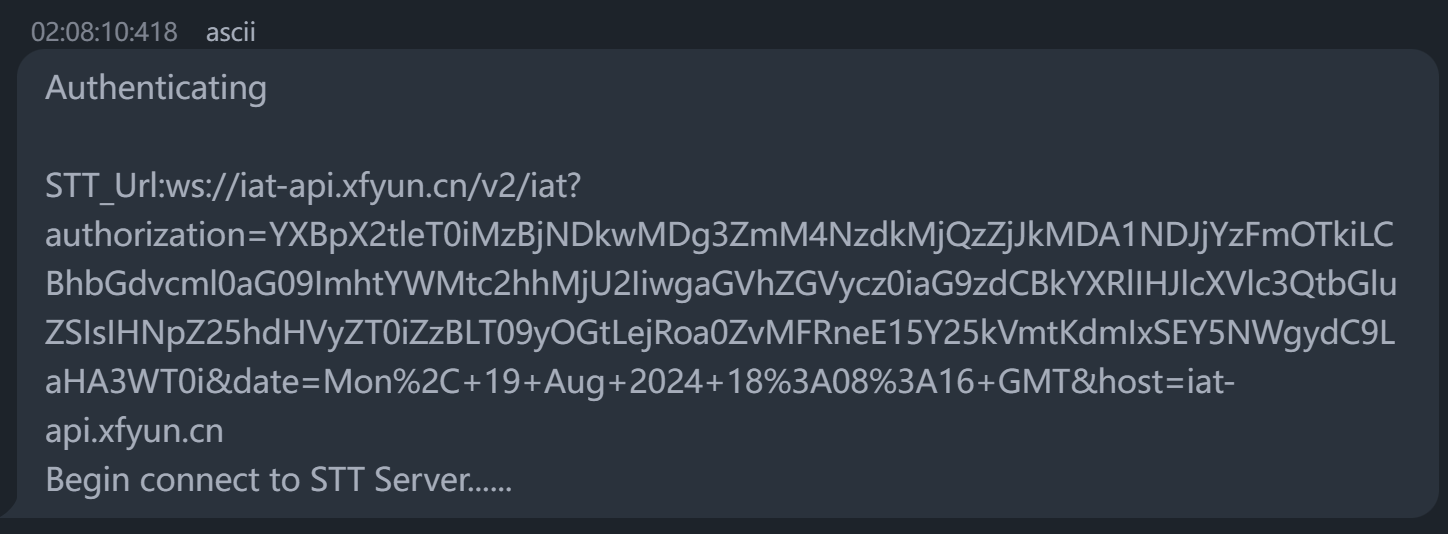
\includegraphics[width=0.4\textwidth]{../img/AuthSuccess.png}
    \caption{鉴权Url}
    \label{fig:AuthorizationUrl}
\end{figure}

\subsubsection{调用LLM API接口进行联网对话}

官方文档中所示示例如下,使用DynamicJson创建动态Json对象,按顺序构造Json即可。

\begin{figure} [H]
    \centering
    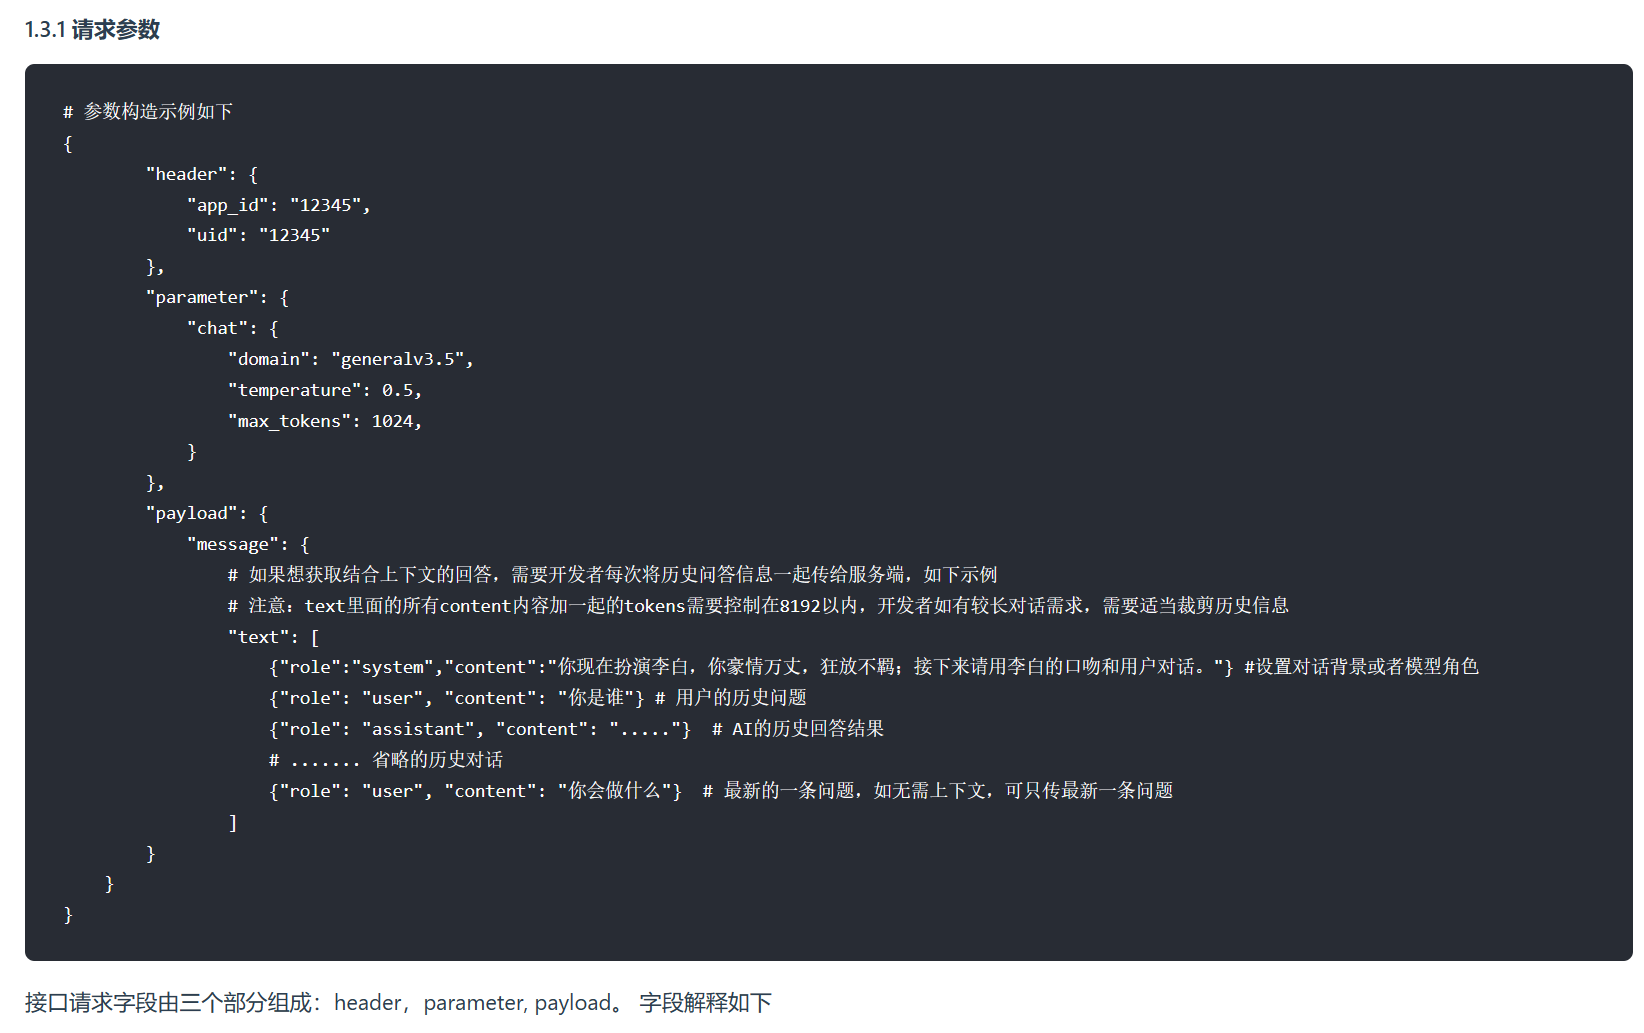
\includegraphics[width=0.6\textwidth]{../img/LLMAPI.png}
    \caption{LLM API参数构造}
    \label{fig:LLMAPI}
\end{figure}

\begin{lstlisting}[language = C++, title = {调用LLM API接口进行联网对话}]

DynamicJsonDocument getParameters(const char *appid, const char *domain, const char *role_set) {
    DynamicJsonDocument data(1500);
    // 构建Json的嵌套对象
    JsonObject header = data.createNestedObject("header");
    JsonObject parameter = data.createNestedObject("parameter");
    JsonObject chat = parameter.createNestedObject("chat");
    JsonObject payload = data.createNestedObject("payload");
    JsonObject message = payload.createNestedObject("message");
    JsonArray textArray = message.createNestedArray("text");
    JsonObject systemMessage = textArray.createNestedObject();
    // 将某些对象赋予值
    header["app_id"] = appid;
    header["uid"] = "1234";
    chat["domain"] = domain;
    chat["temperature"] = 0.6;
    chat["max_tokens"] = 1024;
    systemMessage["role"] = "system";
    systemMessage["content"] = role_set;

    return data;
}
\end{lstlisting}

注意到在$payload \rightarrow message \rightarrow text$中,我们可以向LLM发送多条文本,以实现多轮对话。
故可以创建一个动态数组存储多轮对话的结果,在此可以使用<Vector>,于是有:

\begin{lstlisting}[language = C++, title = {多轮对话实现}]
    // 反序列化:将历史对话 Strings 返回到一个 Json 对象
    for (const auto &jsonStr: historicalDialogue) {
        DynamicJsonDocument tempDoc(512);
        DeserializationError error = deserializeJson(tempDoc, jsonStr);
        if (!error) textArray.add(tempDoc.as<JsonVariant>());
    }
    return data;
\end{lstlisting}

限于代码长度限制,下面给出后续流程的脑图。

\begin{figure} [H]
    \centering
    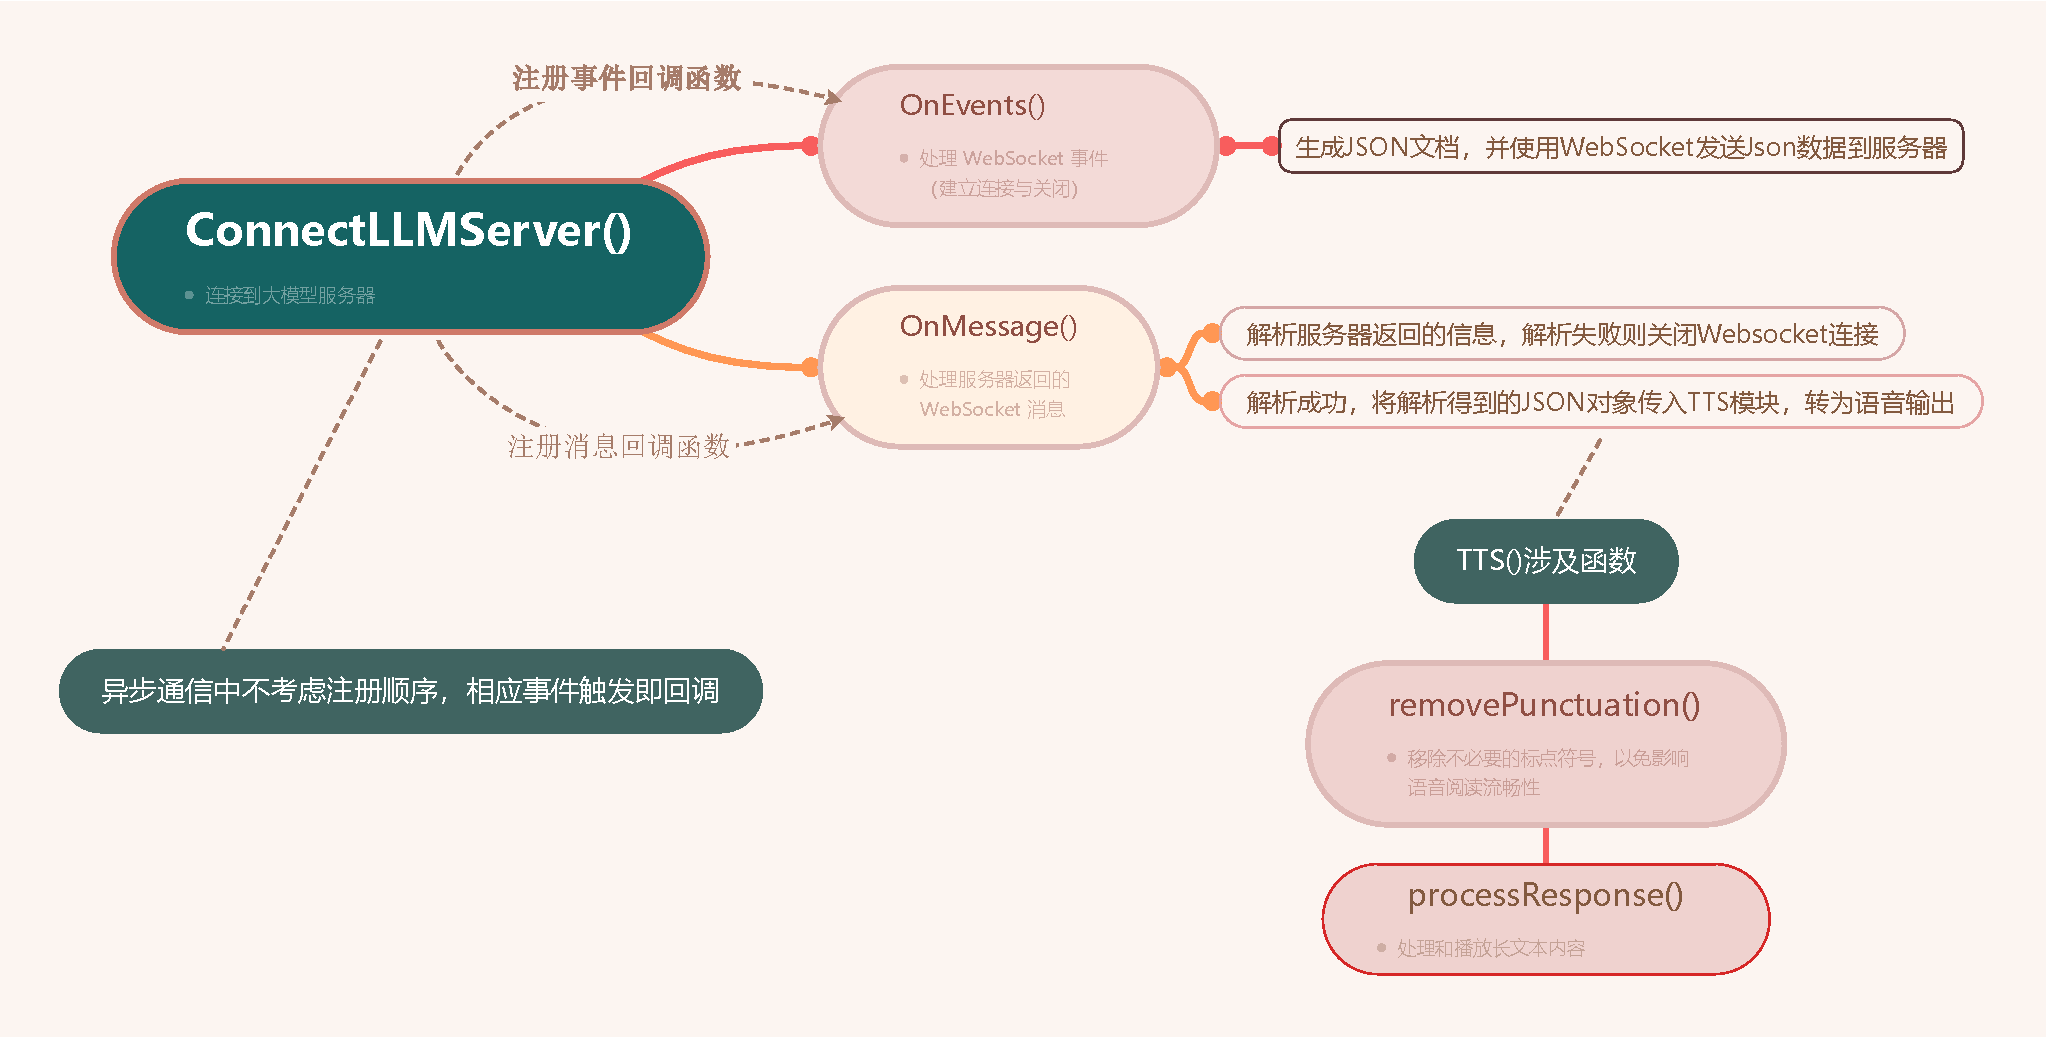
\includegraphics[width=0.9\textwidth]{../img/ConnectLLMServer.pdf}
    \caption{LLM与TTS交互的流程及实现}
    \label{fig:ConnectLLMServer}
\end{figure}

\subsection{基于MQTT协议的物联网搭建}

中国移动的OneNET平台专门为物联网应用开发,我们可以使用ESP32连接到MQTT服务器,之后再构建手机APP来获取数据,真正实现信息互联。

\subsubsection{构建OneNET平台鉴权token}
OneNET平台:\href{https://open.iot.10086.cn/}{\underline{https://open.iot.10086.cn/}}
我使用的是OneJSON数据结构,MQTT协议上传。

将一些基础信息置于此地,后续需要时在这里查看:(鉴权Token在后节获得)
\begin{itemize}
    \item 设备密钥:VzZrREE0T2hYeDZ0dDFQSUZZWWRIZ29yMGxrRUdGY2g=
    \item 设备名称:DHT22
    \item 产品ID:W9TI0JaXlu
    \item 产品Access:8fnx/QsBBf/BUeWpU68j4bG7iwNVm315g+vzc8c
    \item 鉴权Token:version=2018-10-31\&res=products\%2FW9TI0JaXlu\%2Fdevices\%2FDHT22\&et=1759306118\&method=md5
    \item \&sign=JRsZv0peZQOTmr7Eg8lGJg\%3D\%3D
\end{itemize}

在PlatformIO中使用PubSubClient库,可以用于在Arduino框架下实现MQTT通信。下面,通过OneNET平台的官方文档找到了接口:\href{https://open.iot.10086.cn/doc/v5/fuse/detail/919}{\underline{https://open.iot.10086.cn/doc/v5/fuse/detail/919}}

\begin{figure} [H]
    \centering
    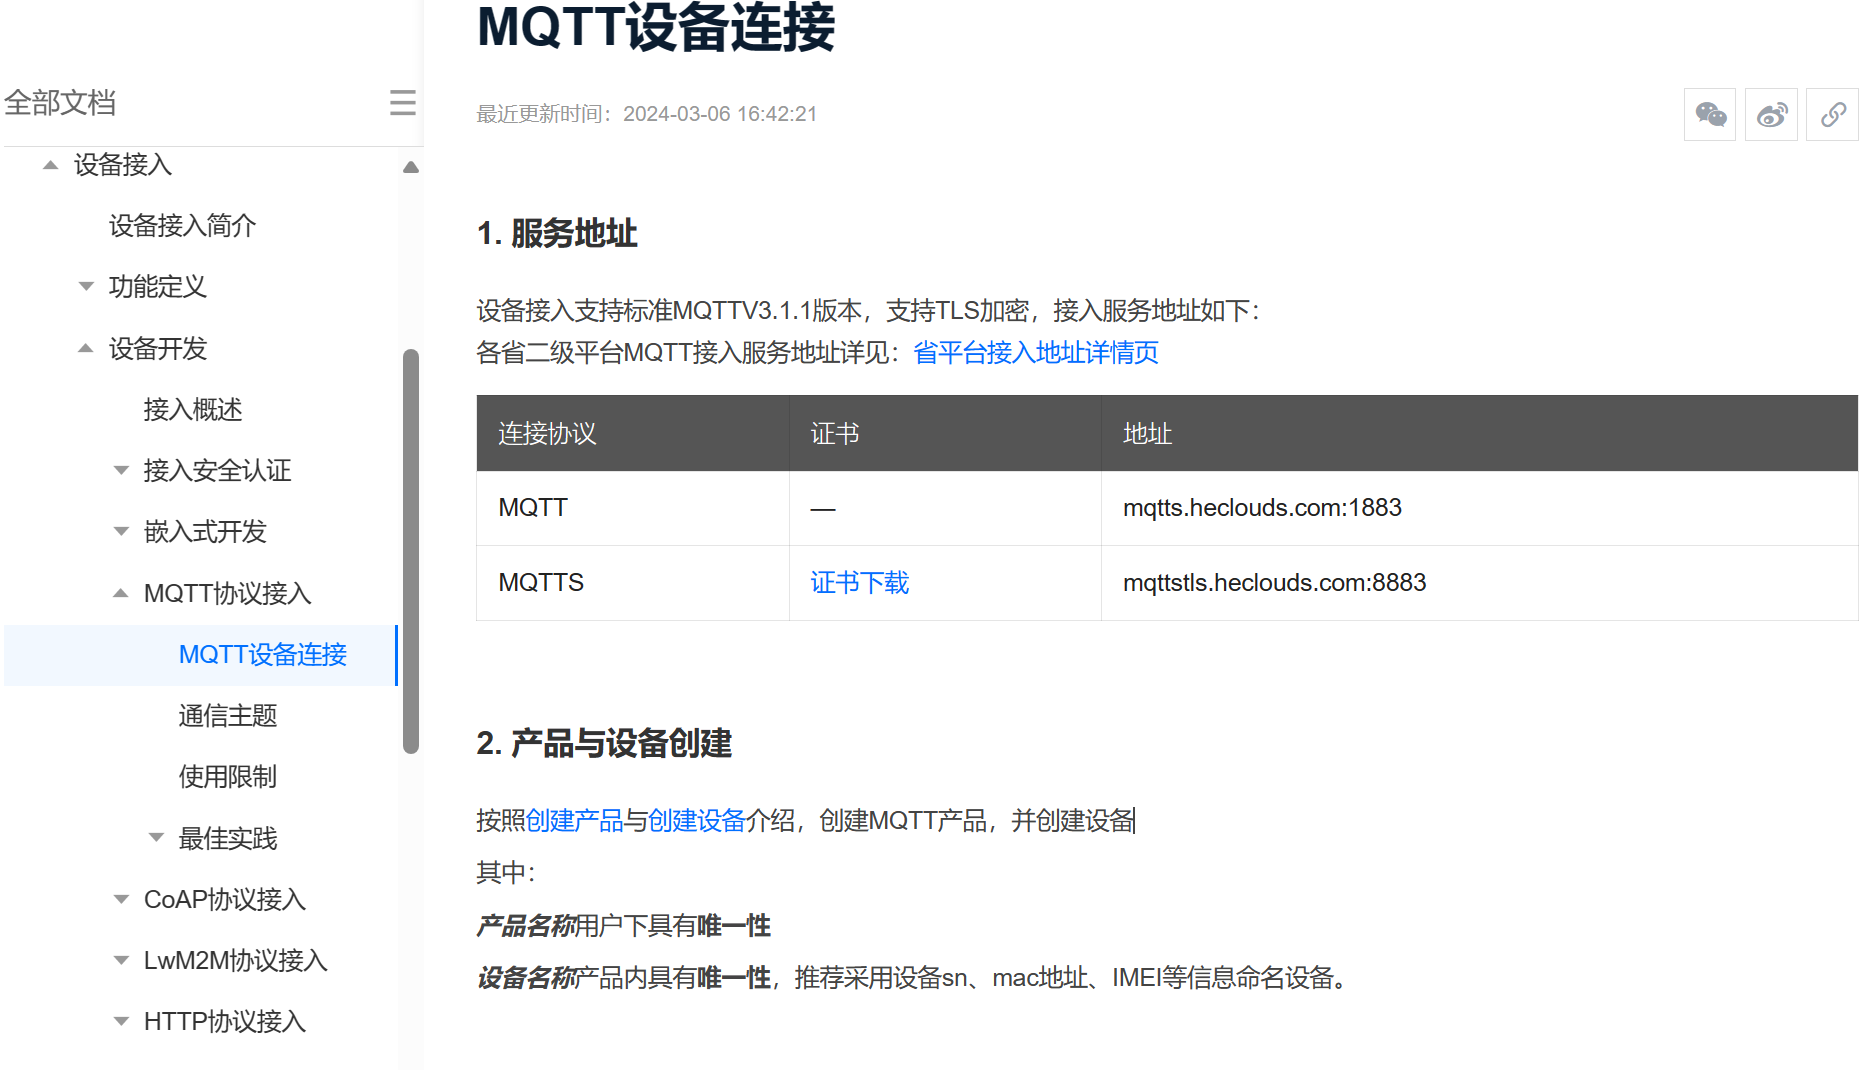
\includegraphics[width=0.7\textwidth]{img/MQTTInit.png}
    \caption{OneNET平台接口}
\end{figure}

按照文档:产品、设备创建时,平台为每类产品、每个设备均分配了唯一的 key,设备登录时需要使用通过key计算出的访问token 来进行访问安全认证。
官方提供了token计算工具,按照res使用场景根据步骤获得token。

\begin{figure} [H]
    \centering
    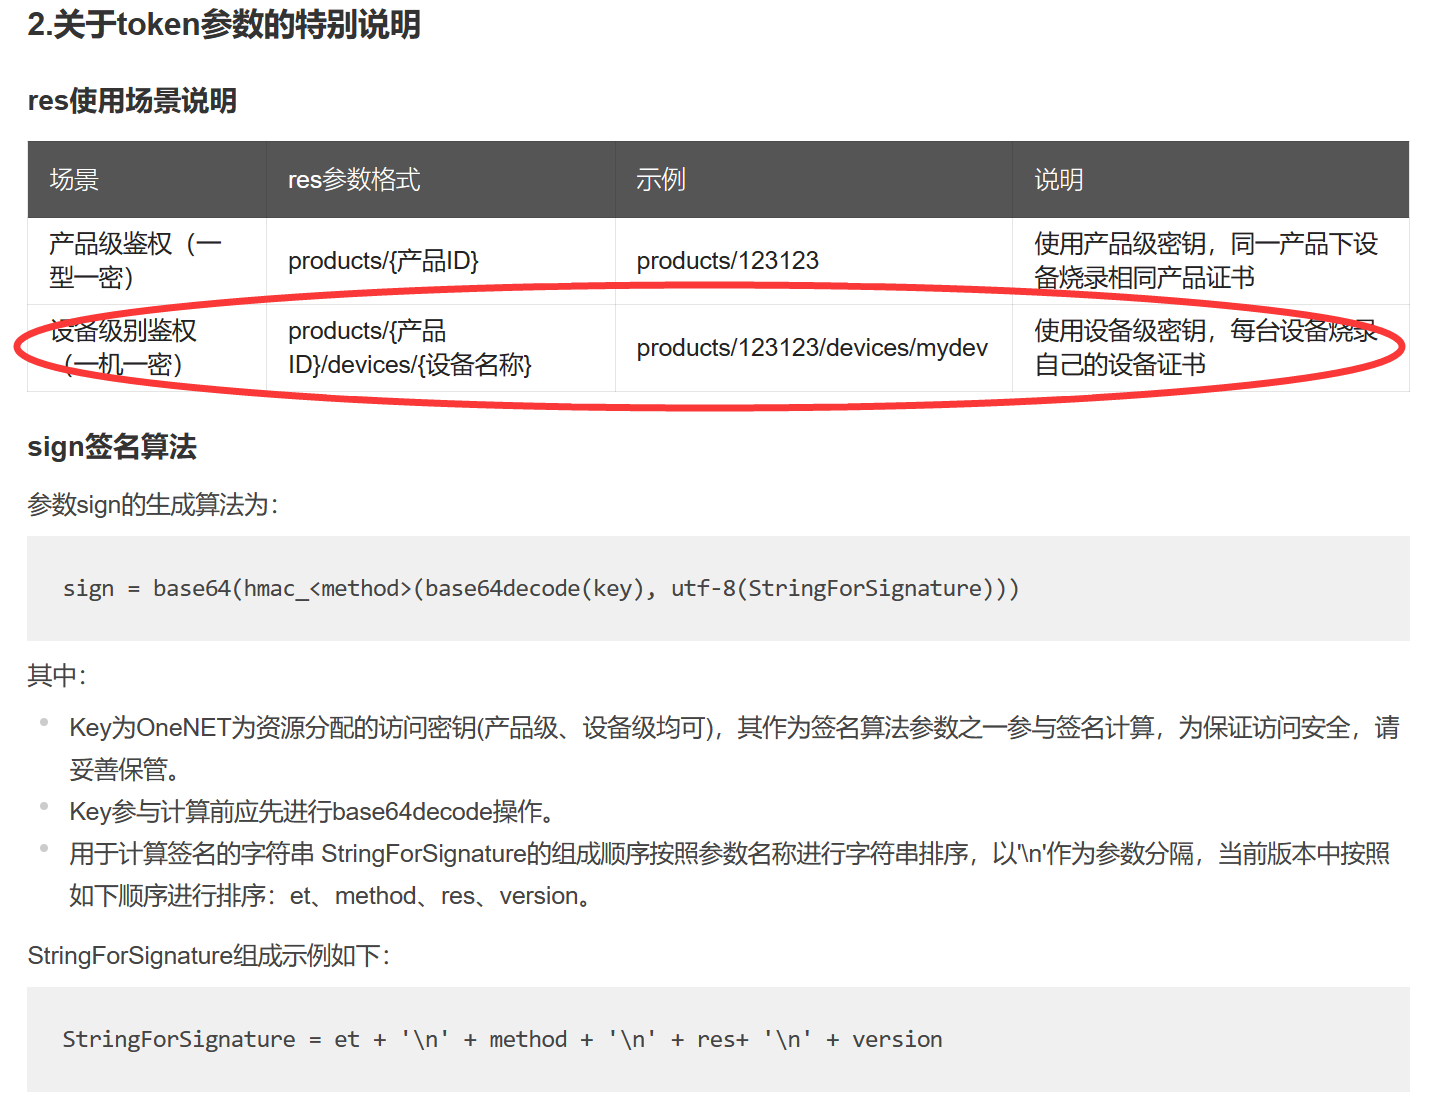
\includegraphics[width=0.5\textwidth]{img/MQTT_Auth.png}
    \caption{OneNET平台token计算}
\end{figure}

在调用讯飞API时我使用的就是Sha-256算法,根据官方文档,支持md5、Sha-1、Sha-256,故我使用Sha-256作为尝试。
注意,官方文档中提到:

\begin{figure} [H]
    \centering
    
\includegraphics[width=0.5\textwidth]{img/Noteet.png}
    \caption{et代表过期时间}
\end{figure}

故使用Unix时间戳转换工具,将到期时间设置为2025年10月1日。

Unix时间戳转换网址为:\href{https://www.jyshare.com/front-end/852/}{\underline{https://www.jyshare.com/front-end/852/}}
,转换得到1759306118。

\begin{figure} [H]
    \centering
    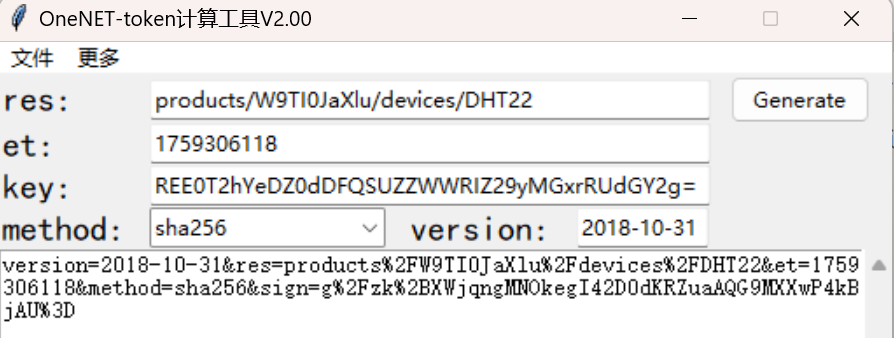
\includegraphics[width=0.5\textwidth]{img/MQTT_sha256.png}
    \caption{计算工具}
    \label{fig:MQTT_sha256}
\end{figure}

\subsubsection{连接到MQTT服务器}

连接到MQTT服务器的关键部分代码如下所示:

\begin{lstlisting}[language=C++, title=MQTT Connect]
    WiFiClient espClient;
    PubSubClient client(espClient);

    void connectOneNet() {
        client.setServer(MQTT_Server.c_str(), MQTT_Port);
        bool isConnected = client.connect(MQTT_Device_ID.c_str(), MQTT_Product_ID.c_str(), MQTT_Token.c_str());
    }

    void loop() {
        client.loop();
    }
\end{lstlisting}

\begin{figure} [H]
    \centering
    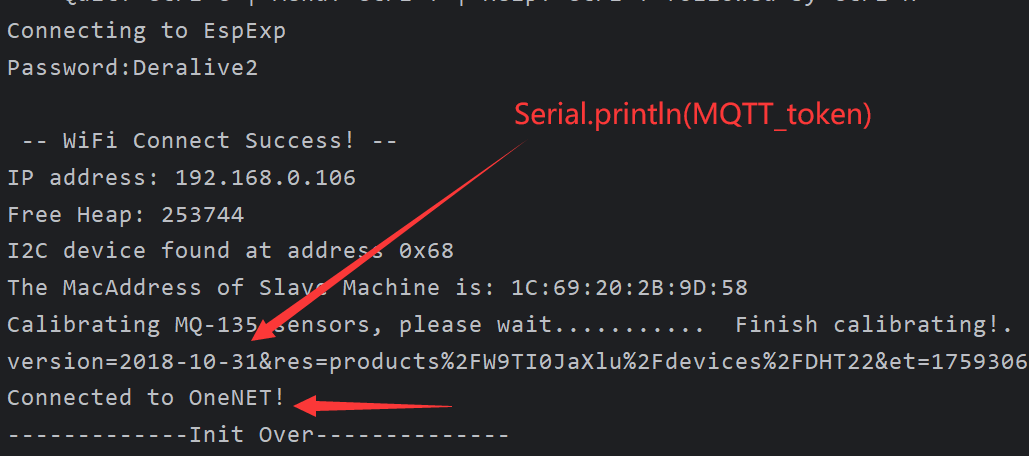
\includegraphics[width=0.5\textwidth]{img/MQTTConnected.png}
    \caption{MQTT服务器连接成功}
\end{figure}

\subsubsection{与MQTT服务器进行数据交互}

连接到服务器后,数据的上传和下载自然成为接下来要攻克的主题。这两部分分别从属于“发布”与“订阅”的操作权限。

\begin{figure} [H]
    \centering
    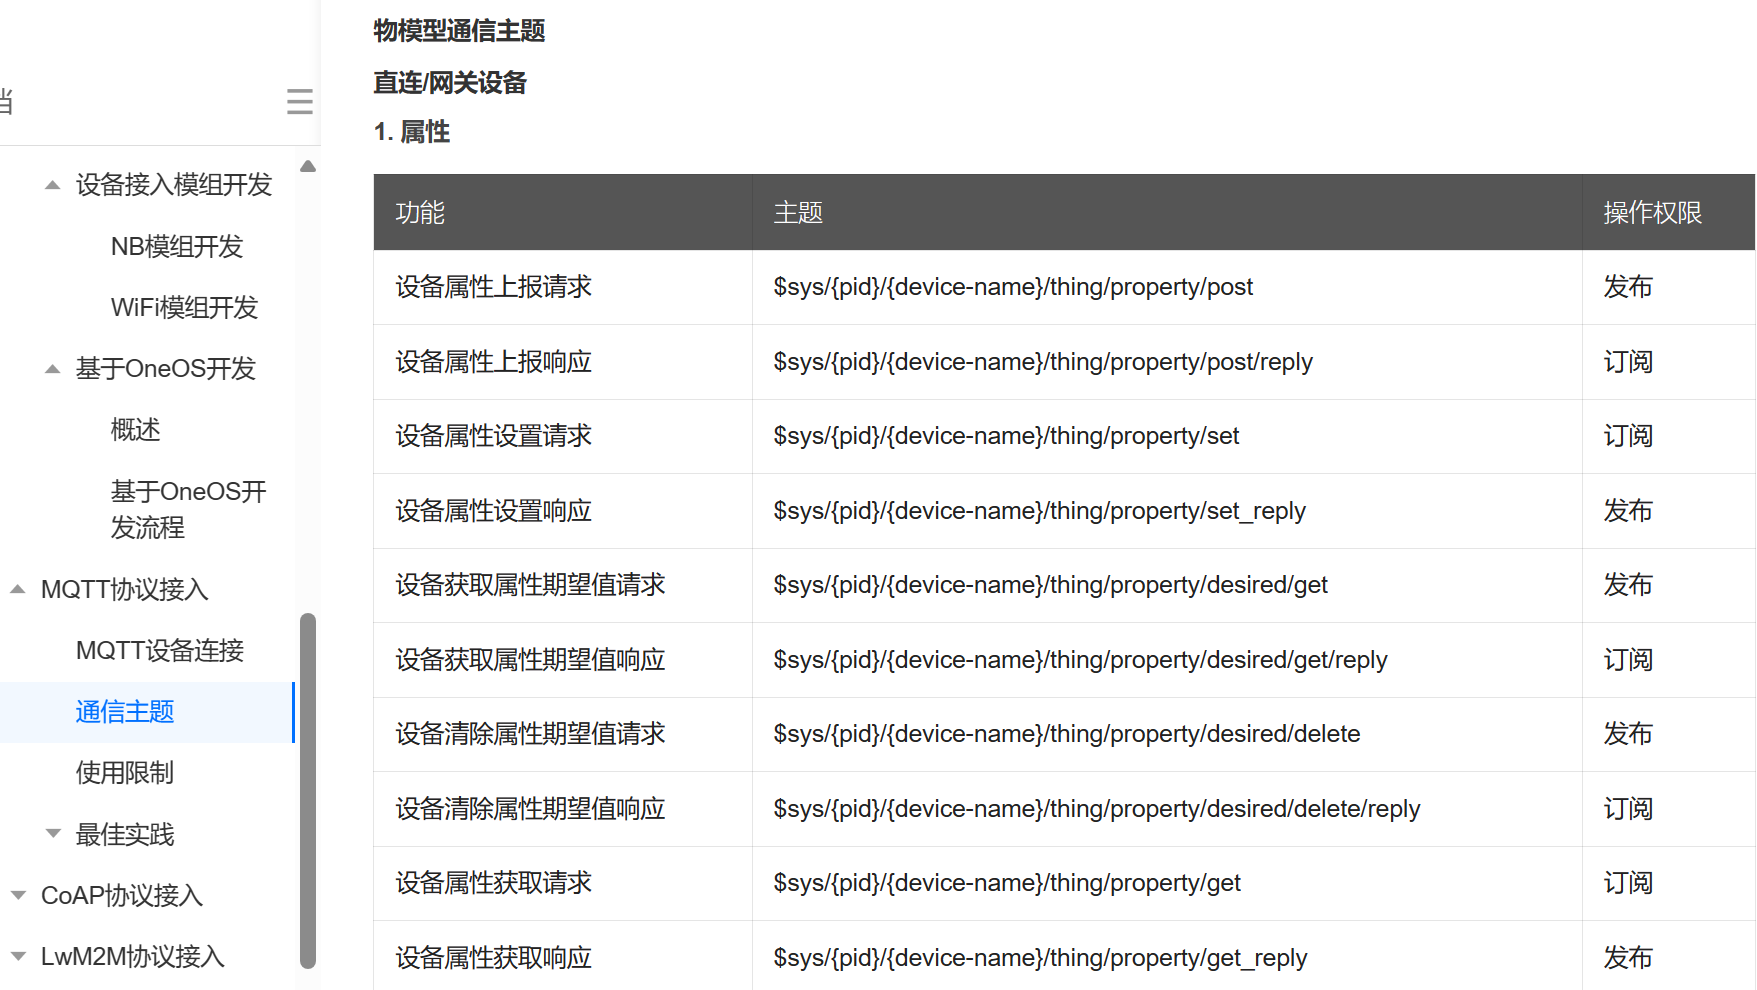
\includegraphics[width=0.6\textwidth]{img/MQTTSubscribe.png}
    \caption{MQTT发布}
\end{figure}

往下翻,需要向服务器传输JSON格式的字符串,如下图所示:

\begin{figure} [H]
    \centering
    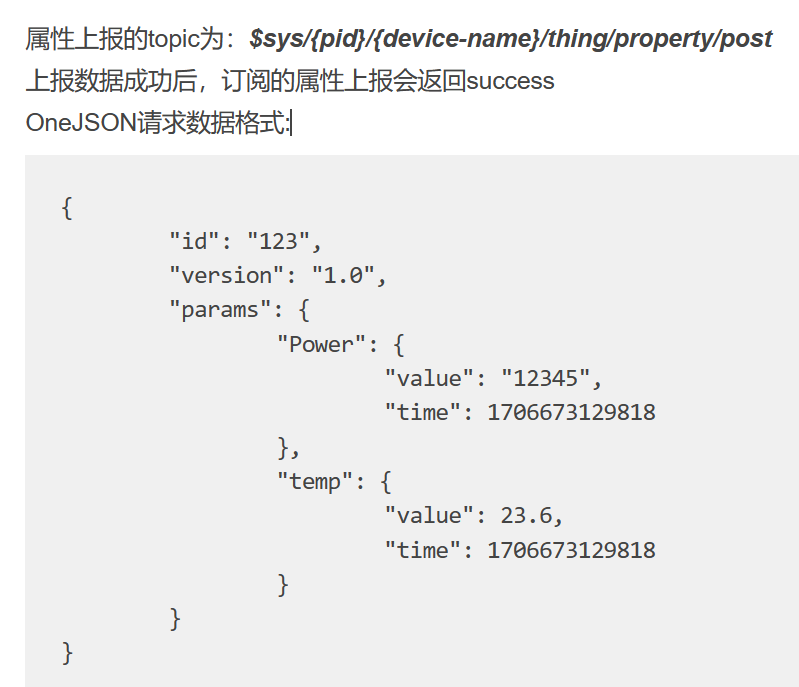
\includegraphics[width=0.3\textwidth]{img/MQTTSendJson.png}
    \caption{MQTT Send Data With JSON Format}
\end{figure}

关键函数如下所示,注意要看物模型通信主题中哪一个是订阅,哪一个是发布。
使用对应的函数\texttt{client.subscribe() 或 client.publish()},同时,设置回调函数mqttCallback(),用于处理服务器返回的数据。
回调函数解析服务器返回的数据,若为 200 则代表数据解析成功。

此处的每一个函数返回的都是boolean类型(可以通过点入函数声明的部分,即在PubSubClient.cpp内查阅),使用返回值来做对应的串口输出,用于提示我是否完成了此次请求。
关键代码如下所示:

\begin{lstlisting} [language=C++, title=MQTT Publish and Subscribe] 
    void connectOneNet() {
        client.setServer(MQTT_Server.c_str(), MQTT_Port);
        client.setCallback(mqttCallback); // 回调函数解析服务器返回的数据,若为 200 则代表数据解析成功

        bool isConnected = client.connect(MQTT_Device_ID.c_str(), MQTT_Product_ID.c_str(), MQTT_Token.c_str());
        bool isSubscribeProperty = client.subscribe(ONENET_TOPIC_PROP_SET); //订阅设备属性设置请求
        bool isSubscribeUpdata = client.subscribe(ONENET_TOPIC_PROP_POST_REPLY); //订阅设备属性上报响应

        if (isConnected) {
            Serial.println(F("Connected to OneNET!"));
        } else {
            Serial.println(F("Failed to connect OneNeT!"));
        }
        // 更多 if,结构一致,为节省篇幅,省略。

        ticker.attach(3,OneNET_Prop_Post); // 使用 Ticker 对象,每隔 3 秒发送一次设备属性上报。
    }
    
    void OneNET_Prop_Post() {
        if (client.connected()) {
            char parameters[256];
            char jsonBuff[256];

            // 构建用来传输至 MQTT 服务器的 JSON 数据
            sprintf(parameters, "{\"temperature\":{\"value\":%.2f},\"humidity\":{\"value\":%.2f}}",dht22Data.temperature,dht22Data.humidity);
            sprintf(jsonBuff,ONENET_TOPIC_PROP_FORMAT,postMessageID++,parameters);
            // 按照文档,#define ONENET_TOPIC_PROP_FORMAT "{\"id\":\"%u\",\"version\":\"1.0\",\"params\":%s}"

            bool isUpData = client.publish(ONENET_TOPIC_PROP_POST, jsonBuff);
        }
    }
    
    void mqttCallback(char* topic, byte* payload, unsigned int length) {
        // 将接收到的消息转换为字符串
        char message[length + 1];
        strncpy(message, (char*)payload, length);
        message[length] = '\0';
    
        // 打印主题和消息内容
        Serial.print("Received message from topic: ");
        Serial.println(topic);
        Serial.print("Message: ");
        Serial.println(message);
    }
\end{lstlisting}

将信息发送至MQTT服务器及服务器接收得到的结果如图所示:

\begin{figure} [H]  
    \centering
    \begin{subfigure}[t]{0.8\textwidth}
        \centering
        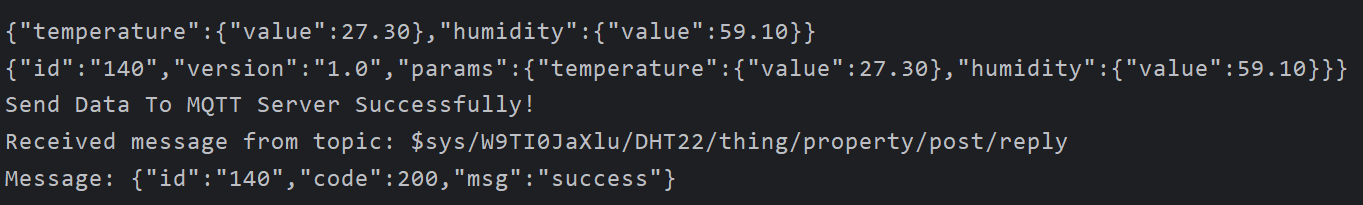
\includegraphics[width=\textwidth]{img/MQTTSendSuccess.png}  
        \caption{将信息发送至MQTT服务器}
        \label{fig:SendToMQTT}
    \end{subfigure}
    
    \vspace{1em}
    
    \begin{subfigure}[t]{0.6\textwidth}
        \centering
        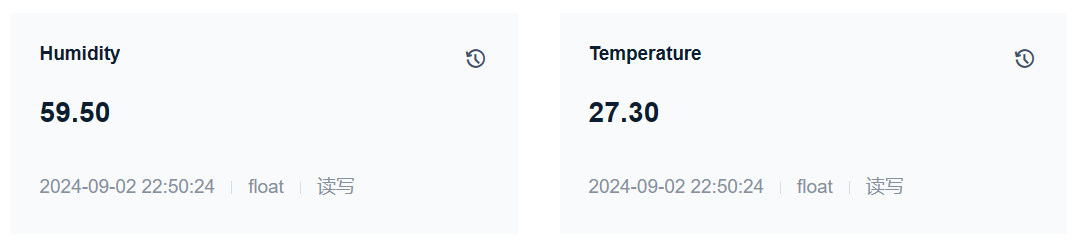
\includegraphics[width=\textwidth]{img/MQTTGetData.png}  
        \caption{OneNET服务器接收到数据}
        \label{fig:OneNETGet}
    \end{subfigure}
    
    \caption{MQTT 发送与接收}
\end{figure}

接下来要做的事情和上面的重复,把其他传感器和想要的数据传输到上面即可。

\begin{figure} [H]
    \centering
    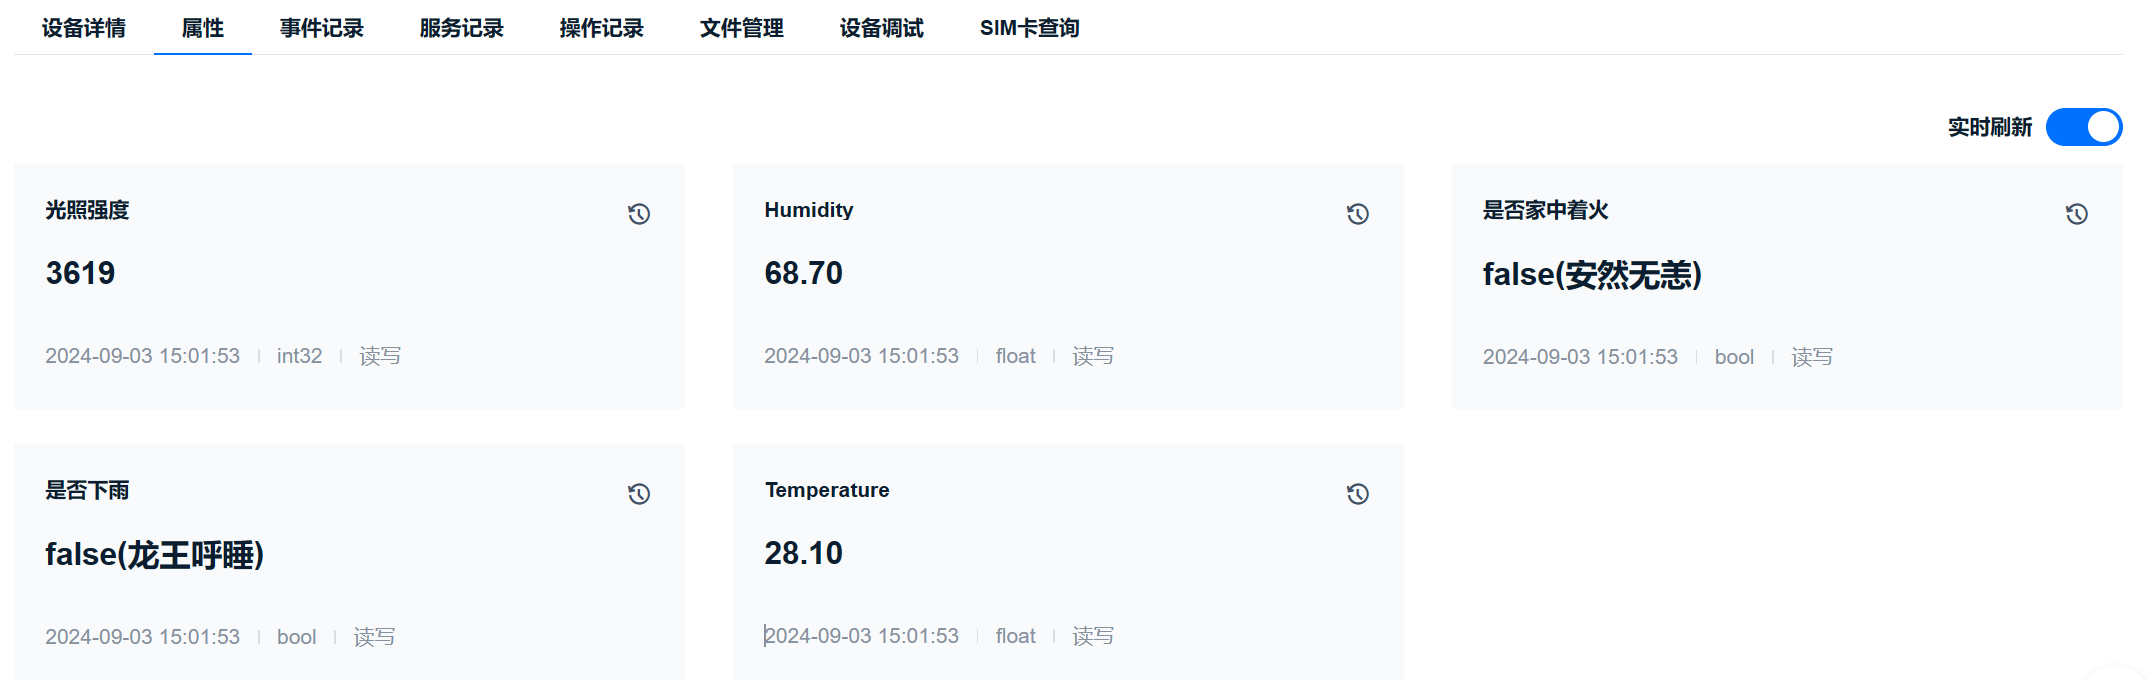
\includegraphics[width=0.5\textwidth]{img/MQTT_Data.png}
    \caption{MQTT服务器接收到的数据}
\end{figure}

\subsection{微信小程序连接MQTT服务器}

\subsubsection{微信小程序连接物联网}

随着安卓平台逐渐没落,多端开发应运而生,此时以Javascript、WXML布局的小程序便可以多端联合开发,而不用担心兼容性问题。
在此,我使用微信开发者工具 Stable 1.06.2407120 进行微信小程序开发,通过远程连接OneNET平台,随时随地,实时显示数据于手机当中。

\subsubsection{构建小程序UI}

基于Nodejs、Javascript语言,使用flex弹性布局,可以使得框架的构建更为简单。
此处的UI图标均采用互联网免费公开资料。

\begin{lstlisting} [language=HTML, caption=微信小程序UI]
    <!-- Title Header -->
    <view class = "container">
        <view class = "head_box">
            <image src = "/images/OneNET.jpg" mode =""/>
        <view>{{title}}</view>
          </view>
    <!-- Weather Module -->
          <view class = "weather_box">
            <view class = "welcome_text">
                  {{welcome}}
            </view>
              <view class = "flex">
                  <view class = "width50">
                    <image src="/images/Weather.jpg" style="width: 200rpx; margin-top: 30rpx; margin-left: 30rpx;" mode="widthFix"/>
                  </view>
                  <view>
                    <view class= "location_text">
                        <image src="/images/located.jpg" style ="width: 20rpx; margin-top: 10rpx;" mode="widthFix"/><text
                        style="font-size: 24rpx;">{{location}}</text>
                    </view>
                    <view>
                        <view class = "temperature_text">
                            {{temperature}}°C
                        </view>
                    </view>
                  </view>
              </view>
          </view>
    <!-- Device Module -->
\end{lstlisting}

再根据实际需要配置实现情况index.wxss, index,js文件,初步实现框架如下所示:

\begin{figure} [H]
    \centering
    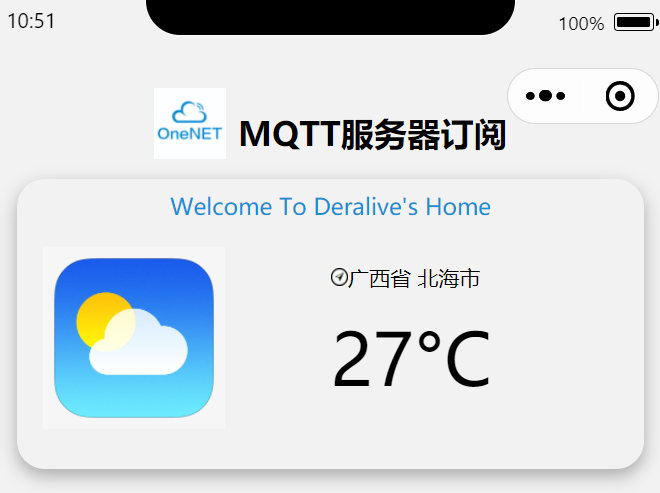
\includegraphics[width=0.3\textwidth]{img/WechatUI.png}
    \caption{微信小程序UI}
    \label{fig:WechatUI}
\end{figure}

根据OneNET平台提供的API,我们需要使用HTTP的GET请求连接到OneNET服务器,这里没办法使用Websocket协议(2024-02更新),

\begin{figure} [H]
    \centering
    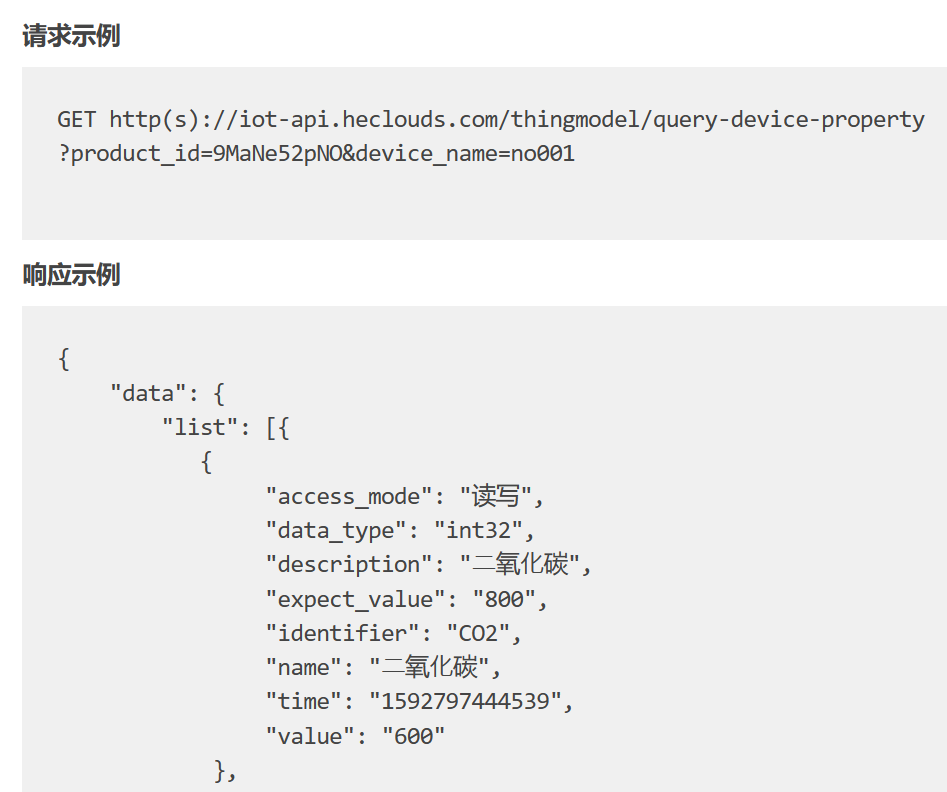
\includegraphics[width=0.35\textwidth]{img/GetMQTTDataHTTPGetExample.png}
    \caption{OneNET GET 请求示例}
    \label{fig:HTTP GET Example}
\end{figure}

按照示例模板,使用API-KEY,根据之前生成的鉴权参数(见图9),生成签名,并将其加入到请求头中,即可完成HTTP请求。

\begin{lstlisting} [language=C++, caption=HTTP GET 请求示例]
    getInfo() {
		let that = this;
		wx.request({
			url: "https://iot-api.heclouds.com/thingmodel/query-device-property?product_id=W9TI0JaXlu&device_name=DHT22",
			header: {
				"authorization": "version=2018-10-31&res=products%2FW9TI0JaXlu%2Fdevices%2FDHT22&et=1759306118&method=md5&sign=JRsZv0peZQOTmr7Eg8lGJg%3D%3D"
			},
			method: "GET",
			success: res => {
				console.log("获取成功", res);
            },
		});
	  },
\end{lstlisting}

获取JSON数据格式如下所示:

\begin{figure} [H]
    \centering
    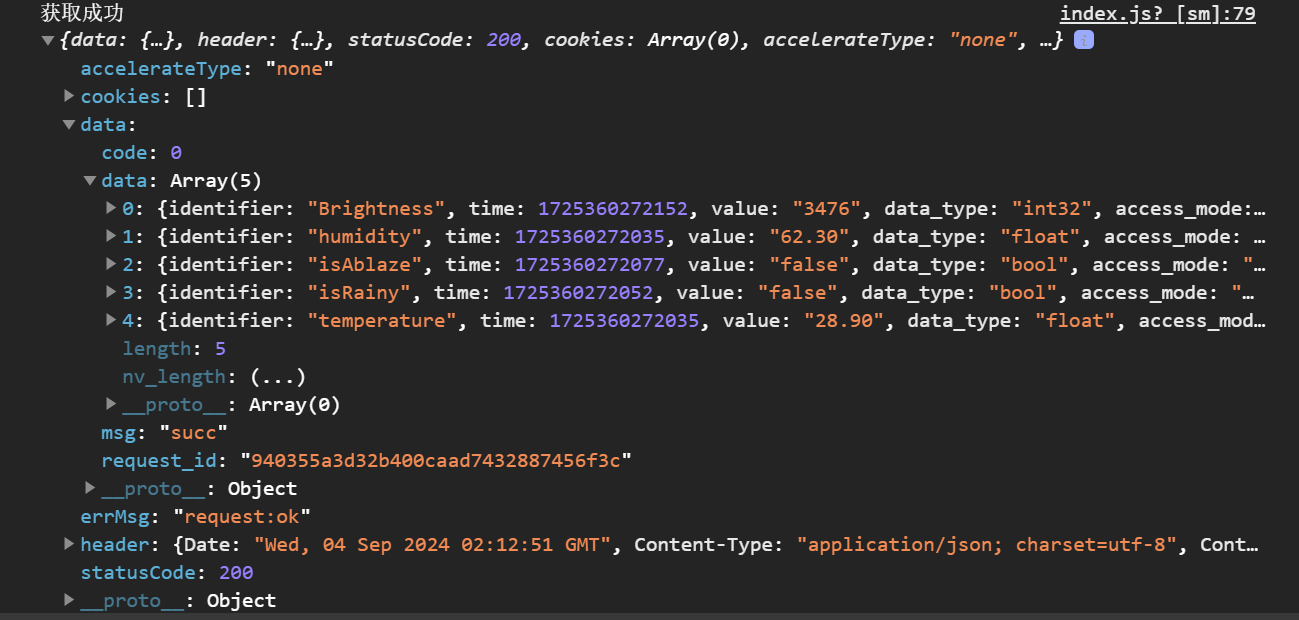
\includegraphics[width=0.45\textwidth]{img/GetMQTTJSON.png}
    \caption{OneNET JSON 数据格式}
    \label{fig:GetMQTTJSON}
\end{figure}

根据data.Array中的参数,每个数组返回的值代表不同的参数,后续只需读取逻辑即可。

\begin{lstlisting} [language=C++, caption=读取JSON数据]
    const sensorList = that.data.sensorList;
    sensorList[0].value = res.data.data[4].value;
    sensorList[1].value = res.data.data[1].value;
    sensorList[2].value = res.data.data[0].value;
    this.setData({
        sensorList: sensorList
    });
\end{lstlisting}

再使用WXML布局,将数据显示在UI上,即可完成微信小程序的连接物联网功能。

\begin{lstlisting} [language=HTML, caption=WXML布局]
    <!-- Sensor UI -->
	<view class = "sensors-system-title">
		传感器设备信息
	</view>
	<view class = "sensors-system">
		<view wx:for="{{sensorList}}" class = "system-info">
			<view class = "sensors-system-box1">
				<image src="{{item.img}}" style = "height: 80rpx; "mode="heightFix"/>
			</view>
			<view class = "sensors-system-box2">
				<view>{{item.parameter}}</view>
				<view>{{item.value}}{{item.unit}}</view>
				<view>{{item.name}}</view>
			</view>
		</view>
	</view>
</view>
\end{lstlisting}

\begin{figure} [H]
    \centering
    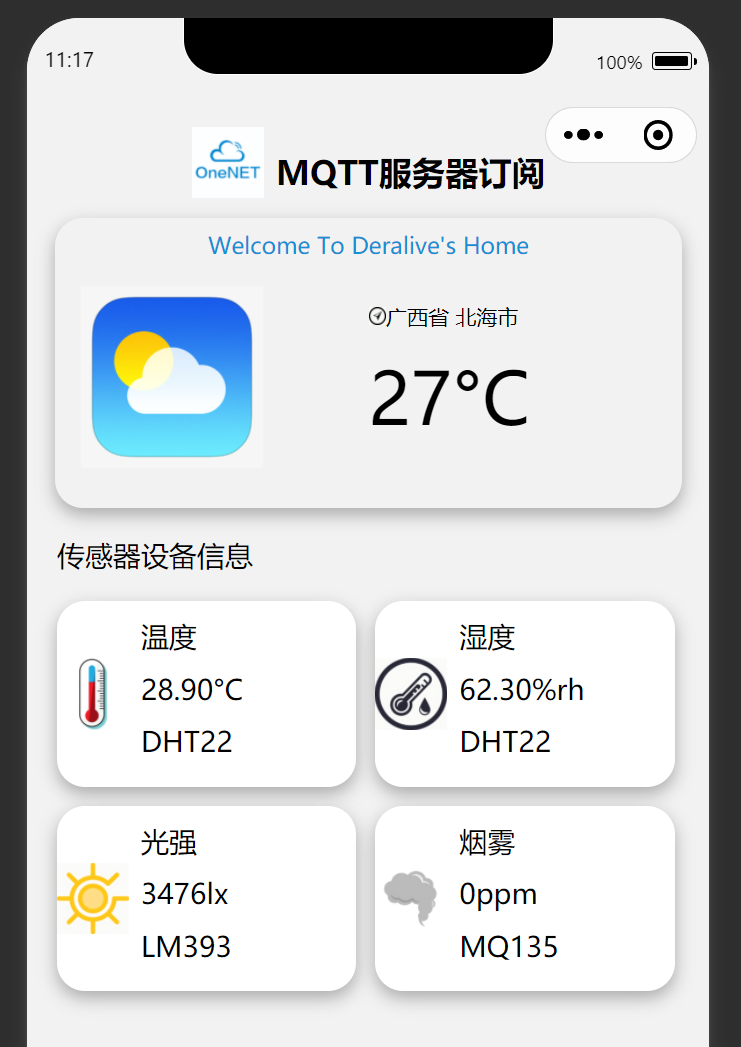
\includegraphics[width=0.2\textwidth]{img/FullUI.png}
    \caption{微信小程序完整UI}
    \label{fig:WechatUI2}
\end{figure}

\subsection{基于ESP-NOW通信协议的使用}

在实现各种功能的过程中,总会发现一块开发板的引脚不够用的情况,此时我考虑使用多块开发板进行开发。
除使用I2C、SPI、UART等协议进行开发板之间的通信之外,本身支持Wifi的ESP32中还有一个由乐鑫公司开发的协议ESP-NOW,
可以无线(即占用更少的引脚)实现两块ESP之间的通信。

我使用ESP32作为主控,主控中调配语音识别大模型,ESP8266中作为从控,调用各种传感器,如DHT11湿温度模块。

通过ESP-NOW协议实现两块ESP之间的通信,读取从控中获取的参数。根据官方手册中的Examples:\href{https://docs.espressif.com/projects/arduino-esp32/en/latest/api/espnow.html?highlight=esp\%20now}{\underline{ESP-NOW.html}},我仿照其代码成功实现了通信。

\subsubsection{获取主板唯一MAC地址}

\begin{lstlisting} [language = C++, title = {获取主板唯一MAC地址}]
    void setup() {
        Serial.begin(115200); // 每一块板的MAC地址是唯一的
        WiFi.mode(WIFI_MODE_STA); // 知道MAC地址后就可以向主机发送信息
        Serial.println(WiFi.macAddress());
    }
\end{lstlisting}

通过上传代码,我将我所需开发板的MAC地址记录在此:

\begin{itemize}
    \item 主板:BC:DD:C2:D0:07:B4
    \item 从控(32):1C:69:20:2B:9D:58
    \item 从控(32E):EC:64:C9:90:6B:74
    \item 从控(32 Side):BC:DD:C2:CD:07:00
    \item 从控(8266):待使用
\end{itemize}

\subsubsection{扫描I2C设备地址}

需要使用IIC协议通信的传感器(如MPU6050),必须需要设备的IIC地址(如\texttt{MPU.begin(0x68,\&Wire);})
使用Wire.h库中的接口扫描,得到 $0x68$。I2C接口不止可以插一根,根据不同的通信地址可以在同一个引脚处插入多个IIC通信。

\begin{lstlisting} [language = C++, title = {扫描I2C设备地址}]
    Wire.begin();  // 初始化I2C总线
    Serial.begin(115200);

    // 扫描所有可能的I2C地址
    for (uint8_t address = 1; address < 127; address++) {
        Wire.beginTransmission(address);
        uint8_t error = Wire.endTransmission();

        if (error == 0) {
            Serial.print("I2C device found at address 0x");
            if (address < 16) Serial.print("0");
            Serial.print(address, HEX);
        }
    }
\end{lstlisting}

\subsubsection{主机(Master)、从控(Slave)代码}

主机(Master)代码:

在根据Examples的运作时,我的ESP-NOW发送数据一直是失败的,
查阅资料后发现要加入一行代码:

\texttt{peerInfo.ifidx = WIFI\_IF\_STA;}

暂不理解为什么其他示例没有这行代码也可以运行,
参考资料:\href{https://esp32.com/viewtopic.php?p=132946}{\underline{https://esp32.com/viewtopic.php?p=132946}}。

\begin{lstlisting} [language = C++, title = {主机(Master)代码}]
// 定义接收到的数据结构
typedef struct struct_message {
    float accelX;
    float accelY;
    float accelZ;
    float temperature;
} struct_message;

struct_message incomingData;

void onDataRecv(const uint8_t * mac, const uint8_t *data, int len) {
    // 将接收到的字节数据解释为结构体类型
    struct_message *receivedData = (struct_message *)data;
}

void setup {
    WiFi.mode(WIFI_STA); // 设置为站点模式
    // 设置对等设备信息
    esp_now_peer_info_t peerInfo;
    peerInfo.channel = 0;
    peerInfo.encrypt = false;
    peerInfo.ifidx = WIFI_IF_STA; // 注意!此步骤一定要有
    // 注册接收回调函数
    esp_now_register_recv_cb(onDataRecv);
}

\end{lstlisting}

从机关键代码,其余部分与主机相似:

\begin{lstlisting} [language = C++, title = {从机(Slave)代码}]
// 目标主机的MAC地址(需要替换为实际的主机MAC地址)
uint8_t masterMACAddress[] = {0xBC,0xDD,0xC2,0xD0,0x07,0xB4};

// 发送回调函数
void onDataSent(const uint8_t *mac_addr, esp_now_send_status_t status) {
    Serial.print("Last Packet Send Status: ");
    Serial.println(status == ESP_NOW_SEND_SUCCESS ? "Delivery Success" : "Delivery Fail");
}

void loop {
    esp_err_t result = esp_now_send(masterMACAddress, (uint8_t *)&myData, sizeof(myData));
}
\end{lstlisting}

\subsubsection{数据传输的关键步骤}

由于在数据传输时,在主机(Master)处只注册了一个回调函数,但从机(Slave)发送的数据有很多种(我定义了不同的结构体来存储变量),
考虑到可能出现结构体对齐问题,不妨将各部分结构体多定义出一个变量,使得接收时可以先判断这个结构体的大小以判断接收到的是什么传感器的数据,接下来再进行数据解析。

\begin{lstlisting} [language = C++, title = {主机读取结构体大小以判断数据来源}]
// 8 字节                          // 12 字节                           // 16 字节
typedef struct DHT22Message {     typedef struct MPU6050Message {       typedef struct MQ5Message {
    float temperature;                float UpAndDown;                      float h2PPM;
    float humidity;                   float LeftAndRight;                   float ch4PPM;
} DHT22Message;                       float temperature;                    float lpgPPM;
                                  } MPU6050Message;                         float flagMQ5;
.......                                                                 } MQ5Message;
\end{lstlisting}

\begin{figure}[H]
    \centering
    \begin{subfigure}[b]{0.42\textwidth}
        \centering
        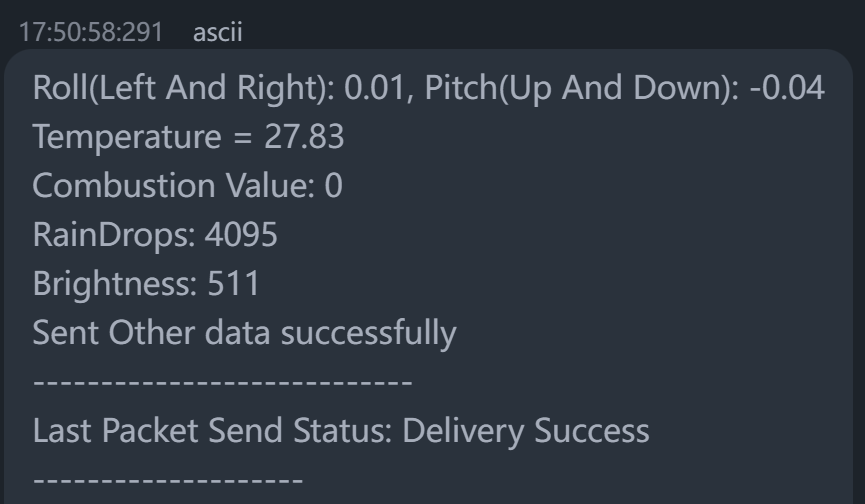
\includegraphics[width=\textwidth]{img/ESP32-Slave-SendData.png}
        \caption{从机发送数据}
        \label{fig:DHT22_active}
    \end{subfigure}
    \hspace{4em}
    \begin{subfigure}[b]{0.325\textwidth}
        \centering
        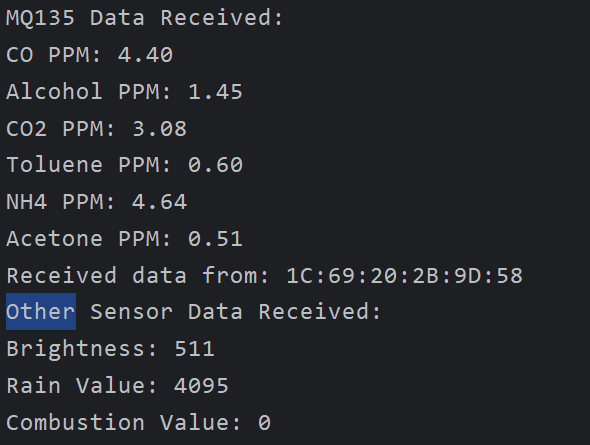
\includegraphics[width=\textwidth]{img/ESP-Master-ReceivedData.png}
        \caption{主机读取数据}
        \label{fig:MPU6050_active}
    \end{subfigure}
    \caption{基于ESP-NOW的数据传输成功}
    \label{fig:combined}
\end{figure}

\subsubsection{ESP与Wifi建立通信}

首先,进入TP-Link路由器的管理界面,室内路由器使用Mesh组网,故使用默认配置地址192.168.0.1。

注意,ESP系列硬件仅支持2.4GHz的无线网络通信,故开启2.4GHz的Wifi。

\begin{figure} [H]
    \centering
    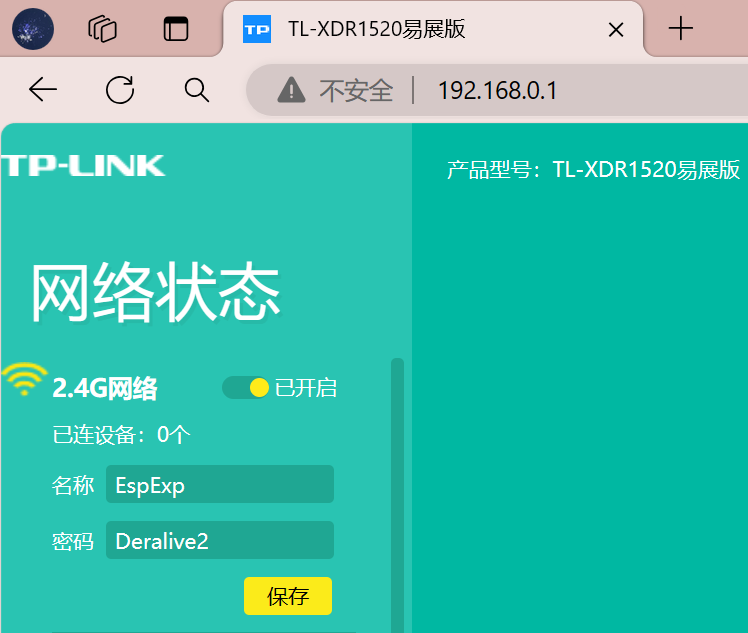
\includegraphics[width=0.3\textwidth]{../img/Wifiset.png}
    \caption{TP-Link路由器管理界面}
\end{figure}

通过Wifi.h库中的接口,进入WifiSTA.cpp查看所有接口(见附件-1),使用Wifi.begin()函数连接到路由器。

\begin{figure} [H]
    \centering
    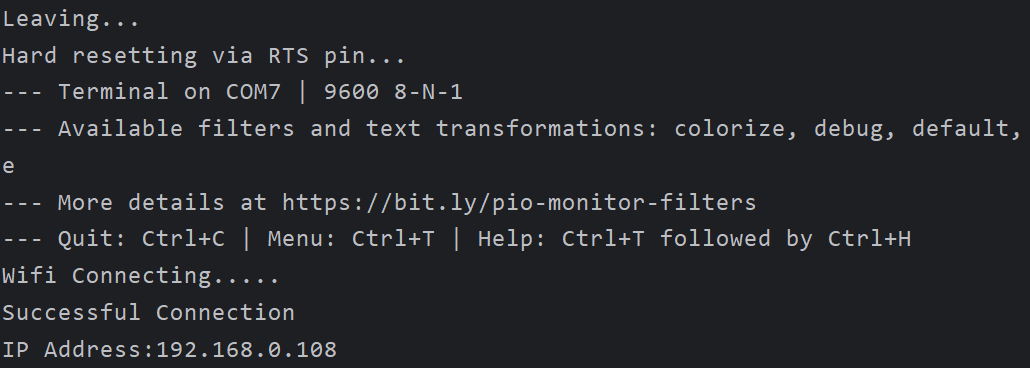
\includegraphics[width=0.5\textwidth]{../img/WifiConnectingSuccess.png}
    \caption{ESP32与Wifi成功建立连接}
\end{figure}

\subsubsection{发送HTTP请求}

心知天气提供免费的天气API查询接口:\href{https://www.seniverse.com/}{https://www.seniverse.com/},先用此进行测试,后续可调用更多API。

\begin{figure} [H]
    \centering
    
\includegraphics[width=0.5\textwidth]{../img/WeatherAPI.png}
    \caption{心知天气API}
\end{figure}

使用HTTPClient.h库,向服务器发送HTTP请求,并接收服务器的响应。使用代码如下所示:

\begin{lstlisting}[language = C++, title = {发送HTTP请求并解析JSON数据}]
  // 创建 HTTPClient 对象并发送 Get 请求
  HTTPClient http;
  http.begin(url+"?key="+key+"&location="+city+"&language="+language+"&unit="+unit);
  int httpCode = http.GET();

  // 获取响应状态码及正文
  Serial.printf("HTTP Status Code: %d", httpCode);
  Serial.print("\n");

  String response = http.getString();
  Serial.println("Response Data:");
  Serial.println(response);

  http.end();

  // 解析 JSON 数据
  DynamicJsonDocument doc(1024);
  deserializeJson(doc, response);

  // 从解析后的 JSON 文档中获取值
  unsigned int temp = doc["results"][0]["now"]["temperature"].as<unsigned int>();
  String info = doc["results"][0]["now"]["text"].as<String>();

  Serial.printf("Daytime temperature: %d\n", temp);
  Serial.printf("Daytime Weather: %s\n", info);
\end{lstlisting}

上传并监视,使用VOFA+ 1.3.10,通信成功,数据解析成功,结果如下图所示:

\begin{figure} [H]
    \centering
    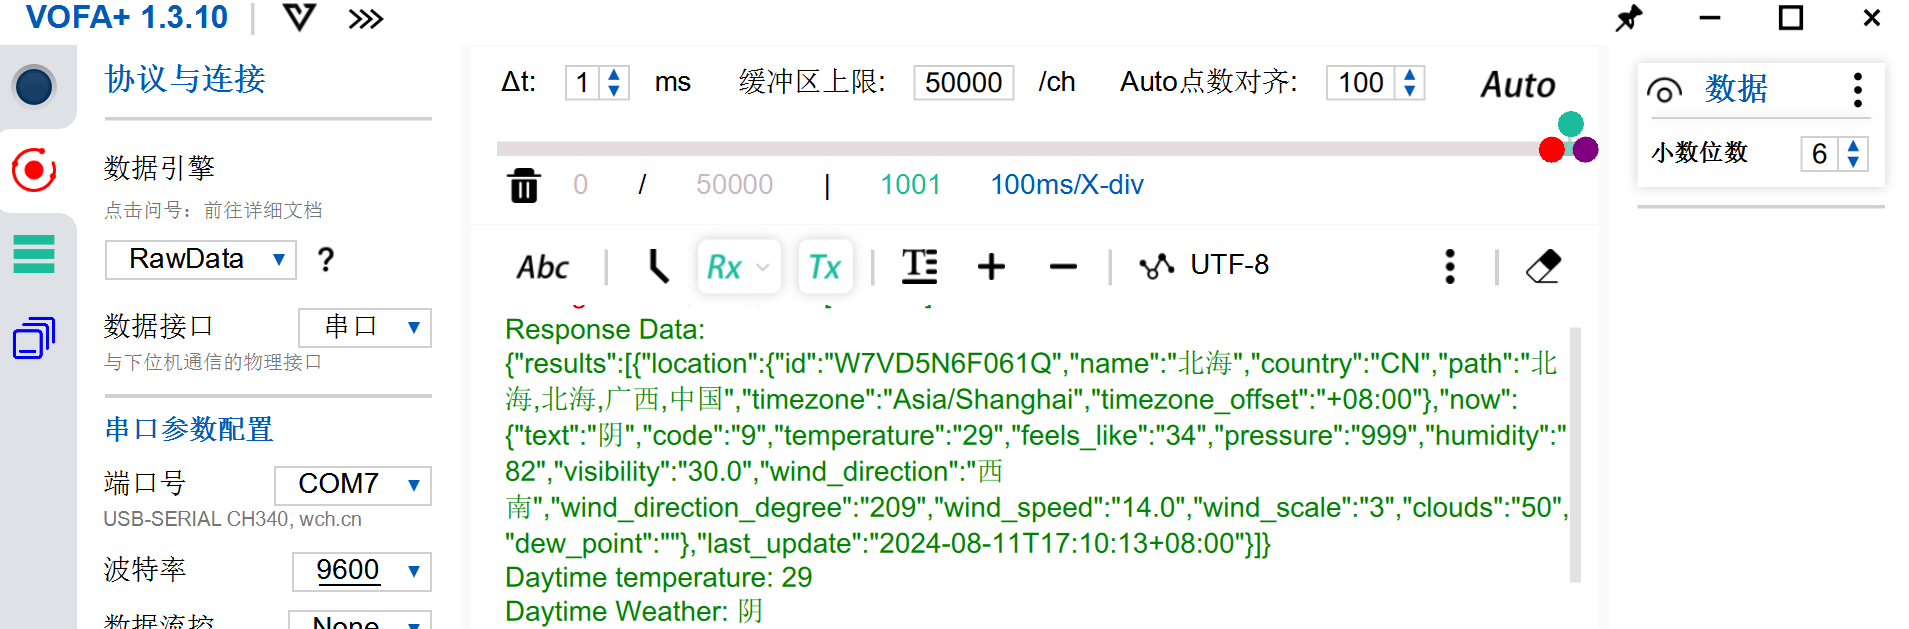
\includegraphics[width=0.7\textwidth]{../img/SerialWeatherInformation.png}
    \caption{天气数据}
\end{figure}

\subsection{多种传感器综合实践}

\subsubsection{DHT22 湿温度传感器}

与MPU6050一致,我们可以构建一个信息结构体,使用ESP-NOW协议将其发送给Master(主机)。

\begin{lstlisting}[language=C++, title=DHT22 Message]
    typedef struct DHT22Message {
        float temperature;
        float humidity;
    } DHT22Message;
\end{lstlisting}

Master收到信息后,解析其中的数据,并与MPU6050的温度进行求平均值处理。
注意,DHT22需要激活信号,在DHT.h代码中查阅发现,使用到了\texttt{pinMode(\_pin, OUTPUT);} 一瞬间来给DHT22发送信号,告诉它需要开始读取并传输信息数据。

成功运行并读取数据的截图(见下图(图\ref{fig:combined}))

\subsubsection{基于卡尔曼滤波的MPU6050姿态解算}

加速度计在静态时解算的姿态的可信度较高,陀螺仪在动态时解算的姿态的可信度较高。
所以需要结合两者的结果进行融合。因为陀螺仪解算的姿态需要积分,随着时间的增加,微小的误差会积分出较大的误差,
这个误差可以通过加速解解算的$roll$,$pitch$减去陀螺仪解算的$roll$,$pitch$,再乘以一个比例系数代替。

参考资料:\href{https://zhuanlan.zhihu.com/p/195683958}{\underline{MPU6050姿态解算2-欧拉角\&旋转矩阵}}

本部分数学知识不在课程学习范围内,故参考了(UP主:地上的感觉还不错)开源程序:

\href{https://www.bilibili.com/video/BV1sL411F7fu}{\underline{学习心得|基于卡尔曼滤波的MPU6050姿态解算}}

同时注意到MPU6050还可以读取环境的温度,故使用该读取温度与$DHT22$读取的温度进行综合,求平均值,能够增大环境温度的可信度。

\begin{figure}[H]
    \centering
    \begin{subfigure}[b]{0.4\textwidth}
        \centering
        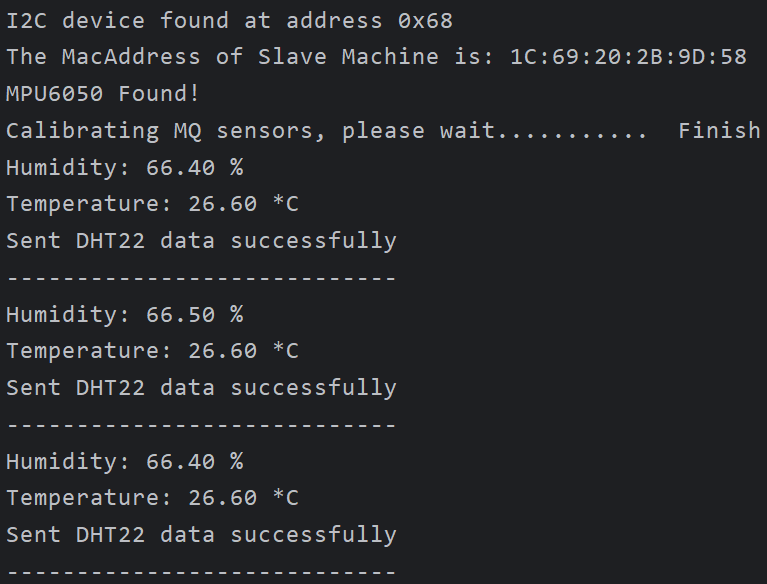
\includegraphics[width=\textwidth]{img/DHT22_active.png}
        \caption{DHT22 运行成功截图}
        \label{fig:DHT22_active}
    \end{subfigure}
    \hspace{4em}
    \begin{subfigure}[b]{0.325\textwidth}
        \centering
        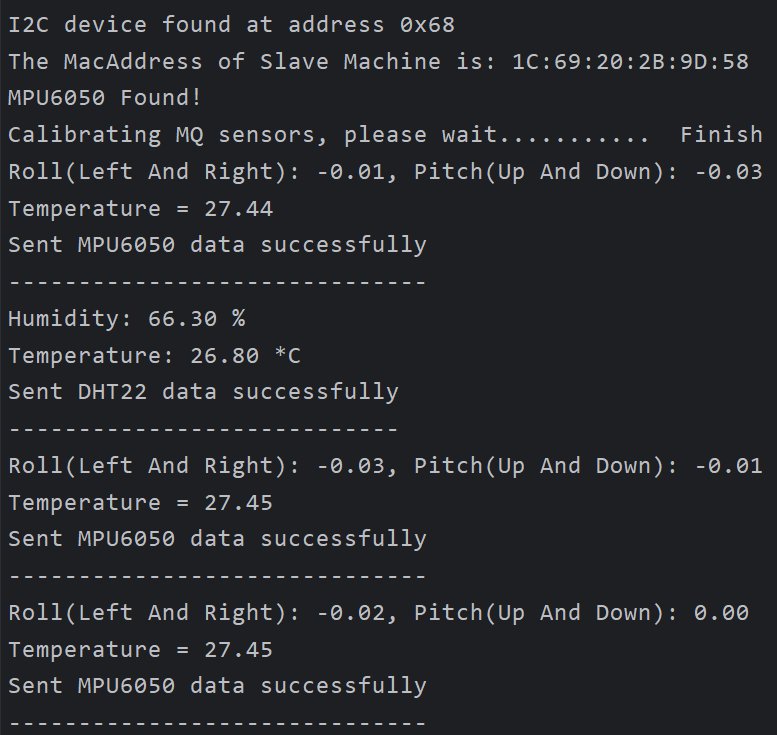
\includegraphics[width=\textwidth]{img/MPU6050_active.png}
        \caption{MPU6050 成功读取偏角}
        \label{fig:MPU6050_active}
    \end{subfigure}
    \caption{DHT22 和 MPU6050 的运行结果}
    \label{fig:combined}
\end{figure}

\subsubsection{MQ系列气体传感器}

MQUnifiedSensor库提供了各种库接口。
初次使用本库时,将ADC引脚定义为ESP32中的GPIO14,报错提示如下所示:

\begin{figure} [H]
    \centering
    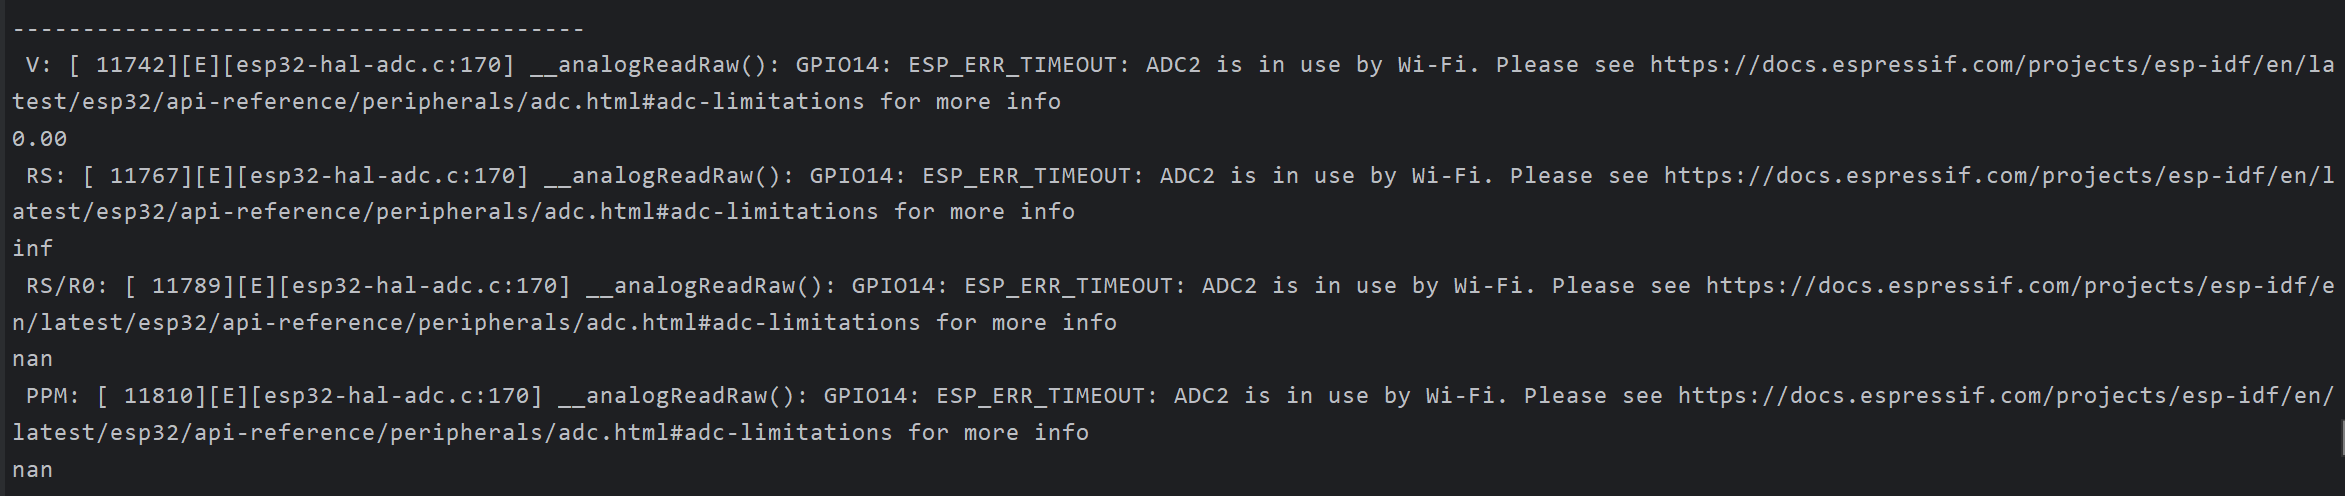
\includegraphics[width=0.8\textwidth]{img/MQ135_error.png}
    \caption{MQ135报错}
    \label{fig:MQ135_error}
\end{figure}

查阅资料后发现,Espressif(ESP32 的制造商)在设计 ESP32 时,
必须在多个功能之间做出权衡。
例如,Wi-Fi 是一个非常关键的功能,它需要稳定的时间控制和电源管理。
因此,当 Wi-Fi 活跃时,它会占用与 ADC2 共享的资源,以确保网络连接的稳定性和性能。

故将ADC模块改用为GPIO32-39即可(见\textcolor{mygreen}{附件}——ESP-Wroom-32开发板的硬件接口)

MQ-135是一种空气质量传感器,用于检测空气中的一氧化碳、氮氧化物、酒精、氨气和烟雾等有害气体。
工作原理是通过化学反应来检测目标气体的浓度,并将结果转换为电信号输出。

对于需要读取不同的气体,需要设置不同的系数(见\textcolor{mygreen}{附件})

故loop代码中应写为:

\begin{lstlisting} [language=C++, title=MQ135 不同气体的读取]
    void loopMQ135() {
        MQ135.update();
    
        // 读取 CO 浓度
        MQ135.setA(605.18);
        MQ135.setB(-3.937);
        float coPPM = MQ135.readSensor();
    
        // 读取 Alcohol 浓度
        MQ135.setA(77.255);
        MQ135.setB(-3.18);
        float alcoholPPM = MQ135.readSensor();
        // ... 重复即可
    }
\end{lstlisting}

参考自官方 MQUnifiedsensor/example/MQ-135-ALL.ino,各参数见\textcolor{mygreen}{附件}。

\begin{figure} [H]
    \centering
    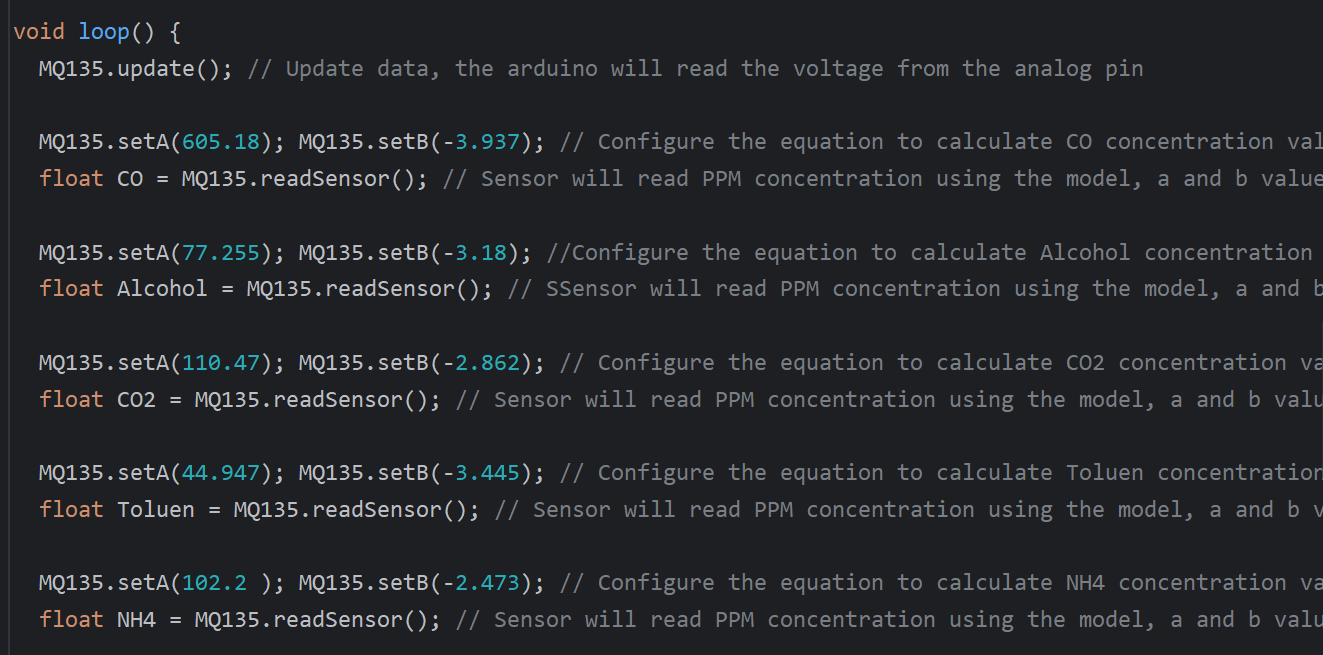
\includegraphics[width=0.5\textwidth]{img/MQ135_Para.png}
    \caption{MQ135 不同气体的系数}
    \label{fig:MQ135_coefficient}
\end{figure}

后续只需要与其他传感器相似,注册回调函数进行数据发送,即可在Master端接收到传感器带来的信息。

同理,我们可以如此操作MQ5传感器,以读取CH4、H2、LPG的PPM值(代表在空气中的浓度)。

\begin{figure} [H]
    \centering
    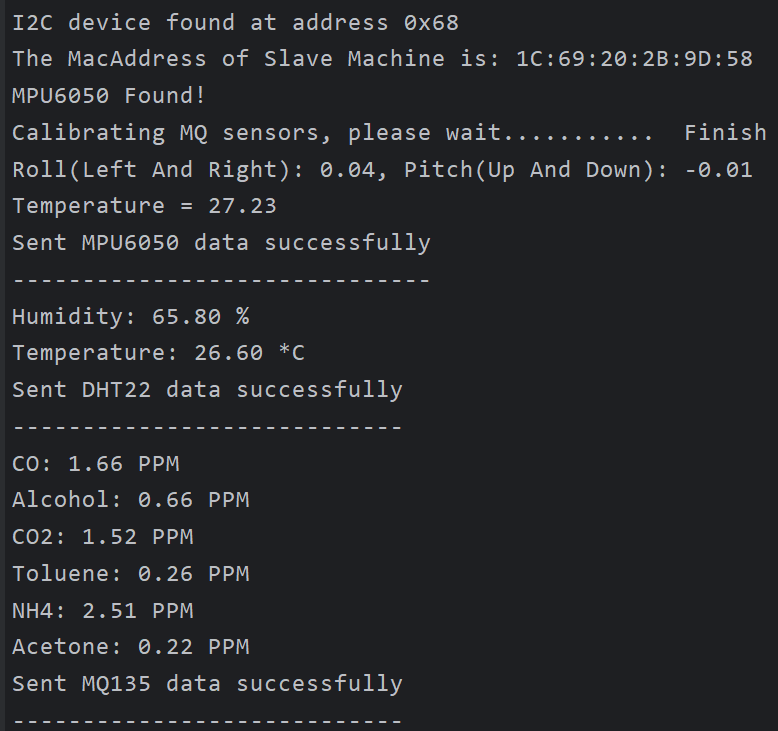
\includegraphics[width=0.4\textwidth]{img/MQ135_active.png}
    \caption{MQ135 成功读取参数}
    \label{fig:MQ135_active}
\end{figure}

\subsubsection{雨滴传感器}

雨滴传感器有两个输出口,分别是AO与DO,为了后续可以开发更多的功能,我们使用AO(Analog Output)输入。

检测是否下雨,如果下雨,则SG90舵机启动,模仿衣架收起的功能。

\subsubsection{LM393光照传感器}

光照传感器同样使用Analog Output模拟输出,为后续开发更多功能打基础。

结合雨滴传感器与光照传感器,还可以设置在夜间自动收回衣服。

\subsubsection{火焰传感器}

检测火焰的强度,在没有火焰时 Analogread() 的值为最大值,火焰越近、燃烧程度越大,得到的模拟信号值越小。

\section{项目心得总结}

在本次课程项目的实践过程中,发现了许多想象中没有出现的问题,并且通过搜索了很多资料,找到了许多方法压缩代码,节省时间,压缩内存空间。例如:

\subsection{编程技巧}

\subsubsection{宏定义与头文件规范}

定义时,我总希望能够使得main.cpp显得不那么冗杂,所以希望开启新的config.h来搜集一切宏定义和全局变量。

搜索资料后发现,头文件通常用于声明变量,而不是定义变量。对于全局变量,应该在头文件中使用extern关键字来声明,然后在一个源文件中实际定义。
并且注释部分的信息(如创建者信息和联系方式)最好放在实现文件(.cpp)中,而不是头文件中。

\subsubsection{宏定义与构造函数接口的冲突}

在使用MQUnifiedsensor.h库时,public接口如下所示:

\texttt{MQUnifiedsensor(String Placa = "Arduino", float Voltage\_Resolution =  5, int ADC\_Bit\_Resolution = 10, int pin = 1, String type = "CUSTOM MQ");}

我在configuration.h中使用\texttt{\#define Voltage\_Resolution 3.3},出现以下报错:

\begin{lstlisting} 
    : note: in expansion of macro 'Voltage_Resolution'
     MQUnifiedsensor(String Placa = "Arduino", float Voltage_Resolution =  5, int ADC_Bit_Resolution = 10, int pin = 1, String type = "CUSTOM MQ");
\end{lstlisting}

报错原因:宏定义是字符替换,这里编译时会变成 "3.3 = 5",故导致编译错误。

\subsubsection{使用"F"宏处理字符串}

F()宏:当使用F()宏时,字符串常量会存储在Flash存储器中,而不是默认的SRAM中。这意味着可以减少动态内存的使用,提高程序的运行效率。
如果不使用F()宏,所有字符串常量(例如"Humidity: ")都会存储在SRAM中。对于内存较少的设备(如Arduino Uno)来说,这会迅速消耗有限的SRAM,导致“内存不足”错误。

参考资料:\href{https://blog.csdn.net/fang\_chuan/article/details/80029546}{\underline{https://blog.csdn.net/fang\_chuan/article/details/80029546}}

使用正则表达式将println\textbackslash("([\textasciicircum"]*)"\textbackslash)替换为println(F("\$1"))即可。

\subsubsection{PlatformIO Libraries 处理方案}

在Arduino IDE上编辑时,库是容易导入的,但对于大文件和项目组织的管理,Arduino IDE的表现令人不满。
于是我选择转向了VSCode + Platform 开发,但Clion中许多VSCode没有的功能更加吸引我,所以转向了Jetbrains家族。

但是初次接触时,我被其复杂性所惊讶,在互联网上搜索相关的导入库的教程也是少之又少,迫不得已到StackOverflow上搜索,并将部分优秀结果自我吸收后作了整理写入了个人的bilibili专栏。

阅读链接:\href{https://www.bilibili.com/read/cv37521671}{\underline{www.bilibili.com/read/cv37521671}}

\subsubsection{ESP32 崩溃后使用 Backtrace 追踪错误代码}

在上传后,有时会出现如下的报错:

\begin{figure} [H]
    \centering
    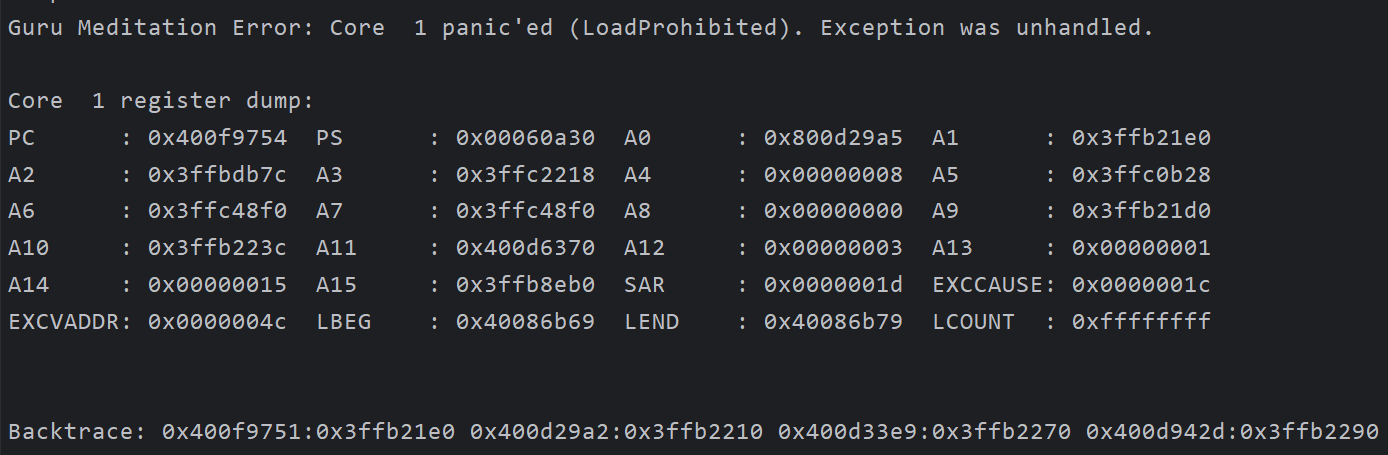
\includegraphics[width=0.5\textwidth]{img/ESP32Error.png}
    \caption{ESP32 崩溃}
    \label{fig:ESP32_crash}
\end{figure}

通过查找资料,可以使用ESP32自带的工具:xtensa-esp32s3-elf-gcc来追溯源代码

命令如下:
\begin{lstlisting}
PS C:\Users\26421\AppData\Local\Arduino15\packages\esp32\tools\xtensa-esp32s3-elf-gcc\esp-2021r2-patch5-8.4.0\bin> .\xtensa-esp32s3-elf-addr2line -pfiaC -e C:\Users\26421\Desktop\Maker\Slave\.pio\build\upesy_wroom\firmware.elf 0x400d29a2:0x3ffb2210 0x400d33e9:0x3ffb2270 0x400d942d:0x3ffb2290
\end{lstlisting}

其中,-e参数指定了elf文件路径,0x400d29a2:0x3ffb2210 0x400d33e9:0x3ffb2270 0x400d942d:0x3ffb2290分别是三个崩溃点的地址。
效果如下所示:

\begin{figure} [H]
    \centering
    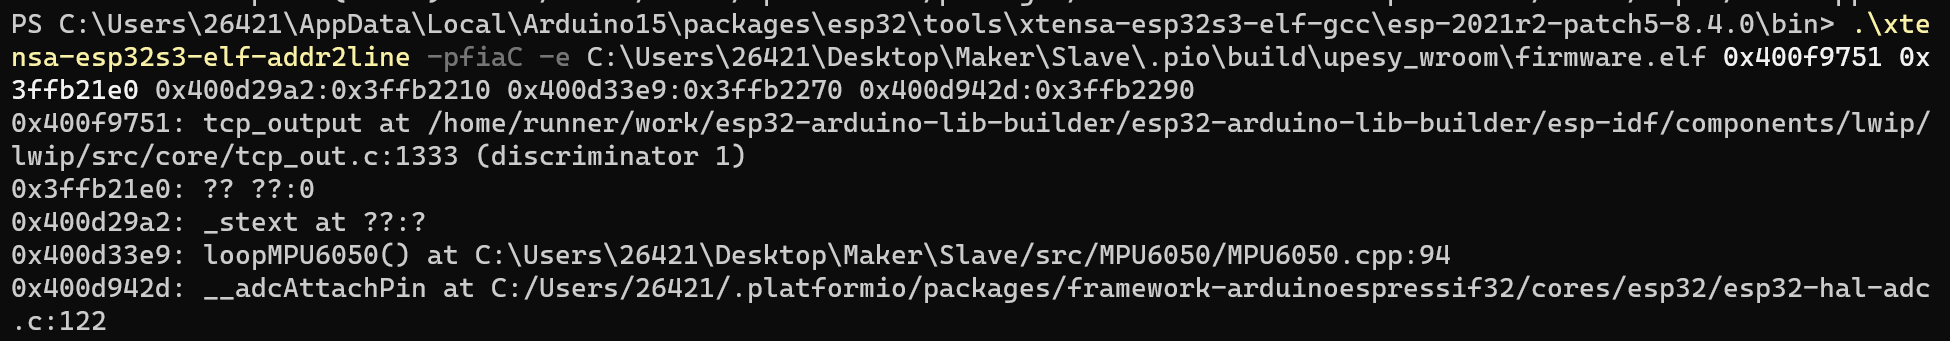
\includegraphics[width=0.7\textwidth]{img/ESP32Backtrace.png}
    \caption{ESP32 Backtrace 追踪错误代码}
    \label{fig:ESP32_backtrace}
\end{figure}


\subsection{个人体验}

本项目乃是我大一一整年做过体量最大、投入最多的项目,很感谢创客实践让我从对嵌入式一窍不通到变得感兴趣。
几乎一切都是从零开始,觉得最有挑战性的部分是涉及到舵机、机械结构的运动学解算,这一部分是需要和外校的同学交流后才知道的。
最觉得有收获的部分是,一点一点地实现语音输入和语音识别、到最后TTS模块的成功运用。

那么,有了语音识别之后,可以再做一些什么呢?不如加一些传感器读取一下个人身体上、房间内、城市里的各种参数吧!
语音识别和输出,显然可以让生活更智能,在项目的构建过程中,也越来越体会到框架的美感。
还有将函数重写时,变得简约易读的程序员之美,在完成一切工作后都体现得淋漓尽致!

为了做一个更漂亮的排版,我去学习了LateX,为了更好的编程和组织文件,我去学习了PlatformIO,最后为了尝试更多东西,跨入了SolidWorks的门槛。
在学习的过程中也接触了很多新概念和新玩法,例如卡尔曼滤波、sha256算法,API的鉴权处理,甚至到ws协议和wss协议的区别。

由于本人在家中尝试搭建家中的路由器组网,所以对网络的了解也更深了一层,能够很快切入ESP32的$AC+AP$模式,甚至有了用ESP32构建Mesh网络的想法。

当然,由于很多部分是第一次探索,搜索了很多资料,也不缺少对各种大模型的使用,但在使用大模型的同时,我将大模型部署到了本地,也许这本身更让人愉悦。
为什么要去实现本来看起来很困难的事情,因为山就在那里。

\subsection{未来设想}

CSI(Channel State Information)用于描述无线通信中的信道特性,可以反映出无线信号在传播过程中受到的多径、衰减、干扰等影响。CSI 在 Wi-Fi 系统中广泛应用,尤其是基于 OFDM(正交频分复用)技术的 Wi-Fi 标准,如 802.11n/ac/ax。
在这些标准中,CSI 可以用于优化传输性能、定位和环境感知等应用。

南京大学无线感知前沿技术论坛在8月1日分享了CSI的前沿研究成果,有望实现毫米级的动态感应。
参考链接:\href{https://www.bilibili.com/video/BV1Cv411q7Cz}{\underline{https://www.bilibili.com/video/BV1Cv411q7Cz}}
,这一部分已有人通过算法实现,原理如同切割磁感线一般,可以通过Wifi强度在人为动作后感应信道的变化,从而读取人类活动,应用前景广泛,将来我很可能从事这方面的研究。

参考链接:\href{https://www.bilibili.com/video/BV1cGHreYEzB}{\underline{用 ESP32-S3 和 CSI 技术打造人体感知风扇}}

\begin{figure} [H]
    \centering
    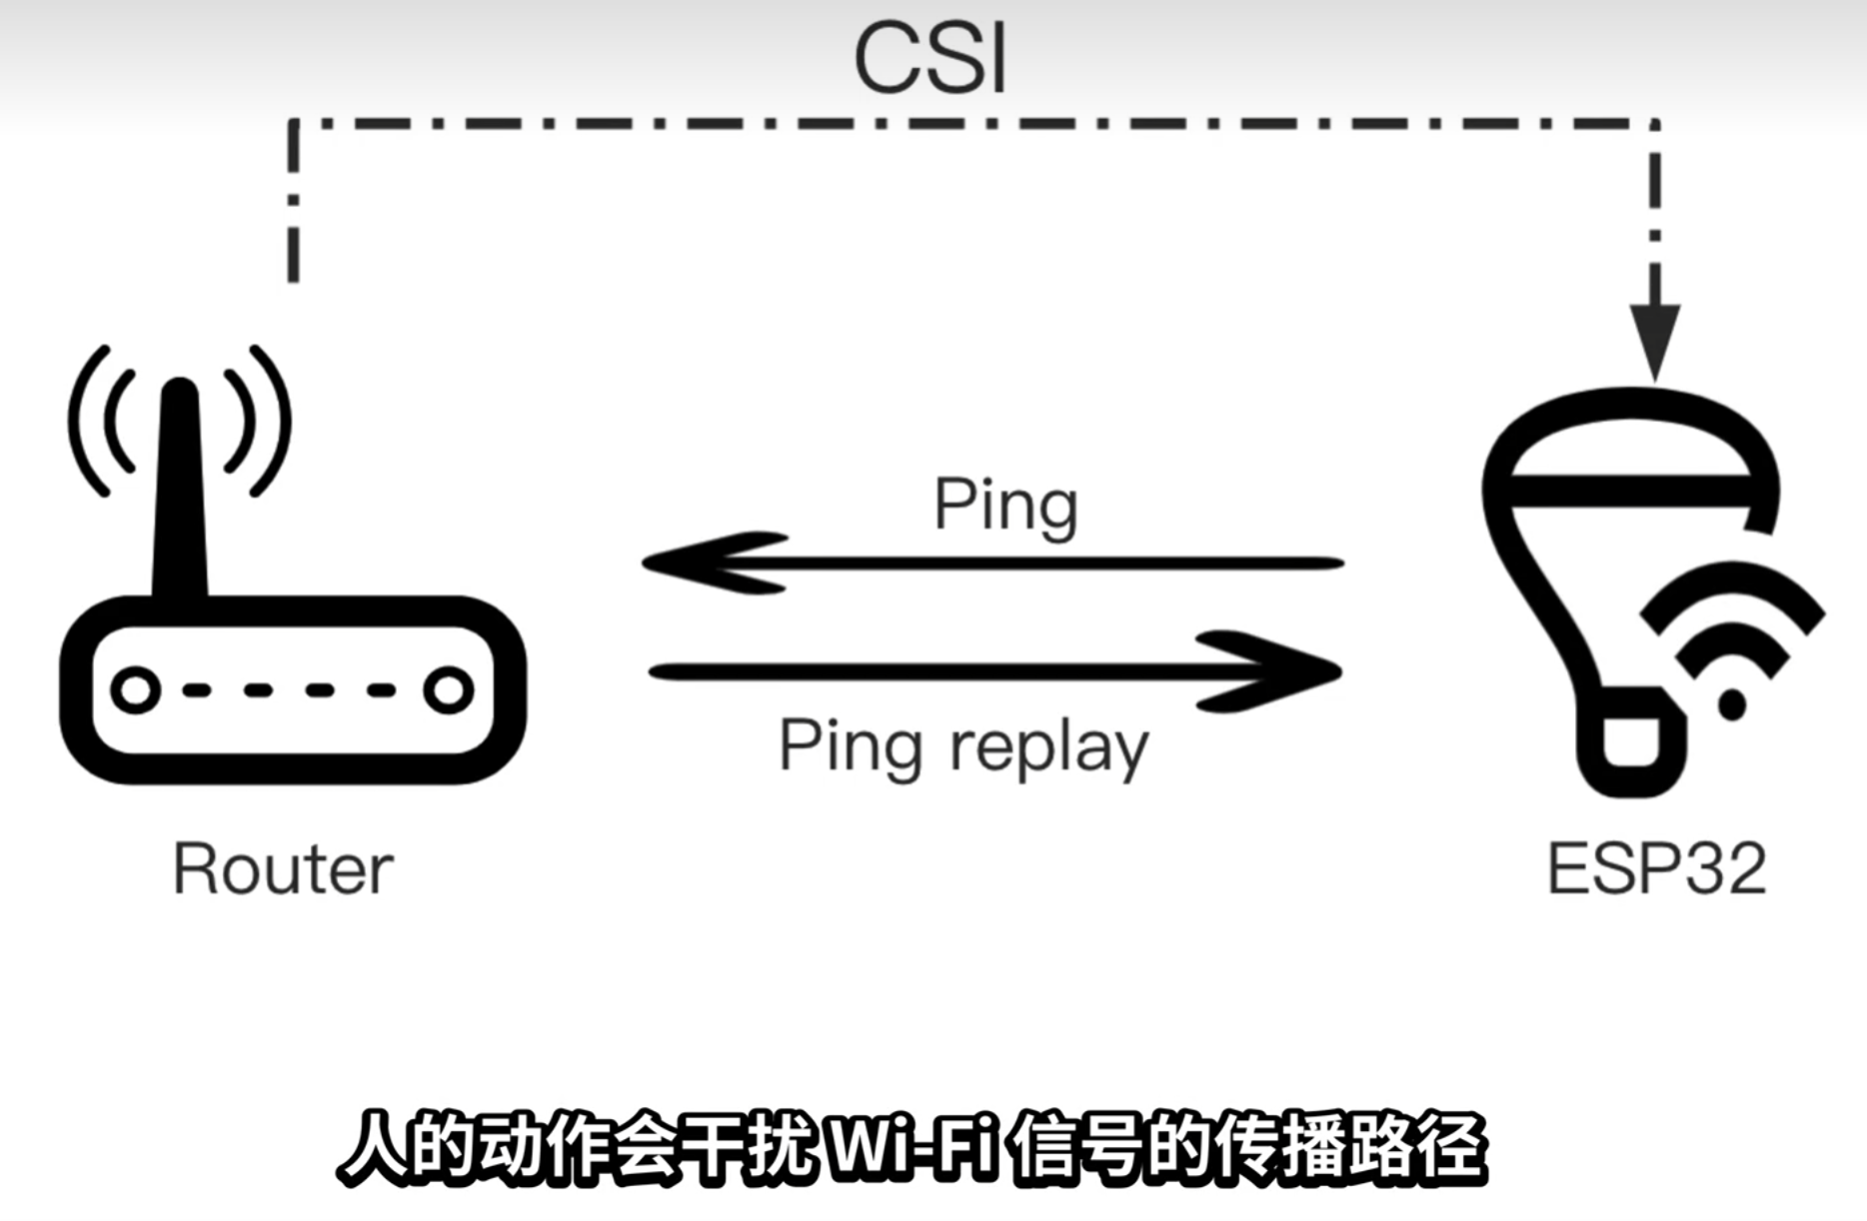
\includegraphics[width=0.4\textwidth]{img/CSI.png}
    \caption{CSI与ESP32-S3结合示意图}
    \label{fig:CSI}
\end{figure}

\newpage{}

\section{附录}


\subsection{项目布局及构建}

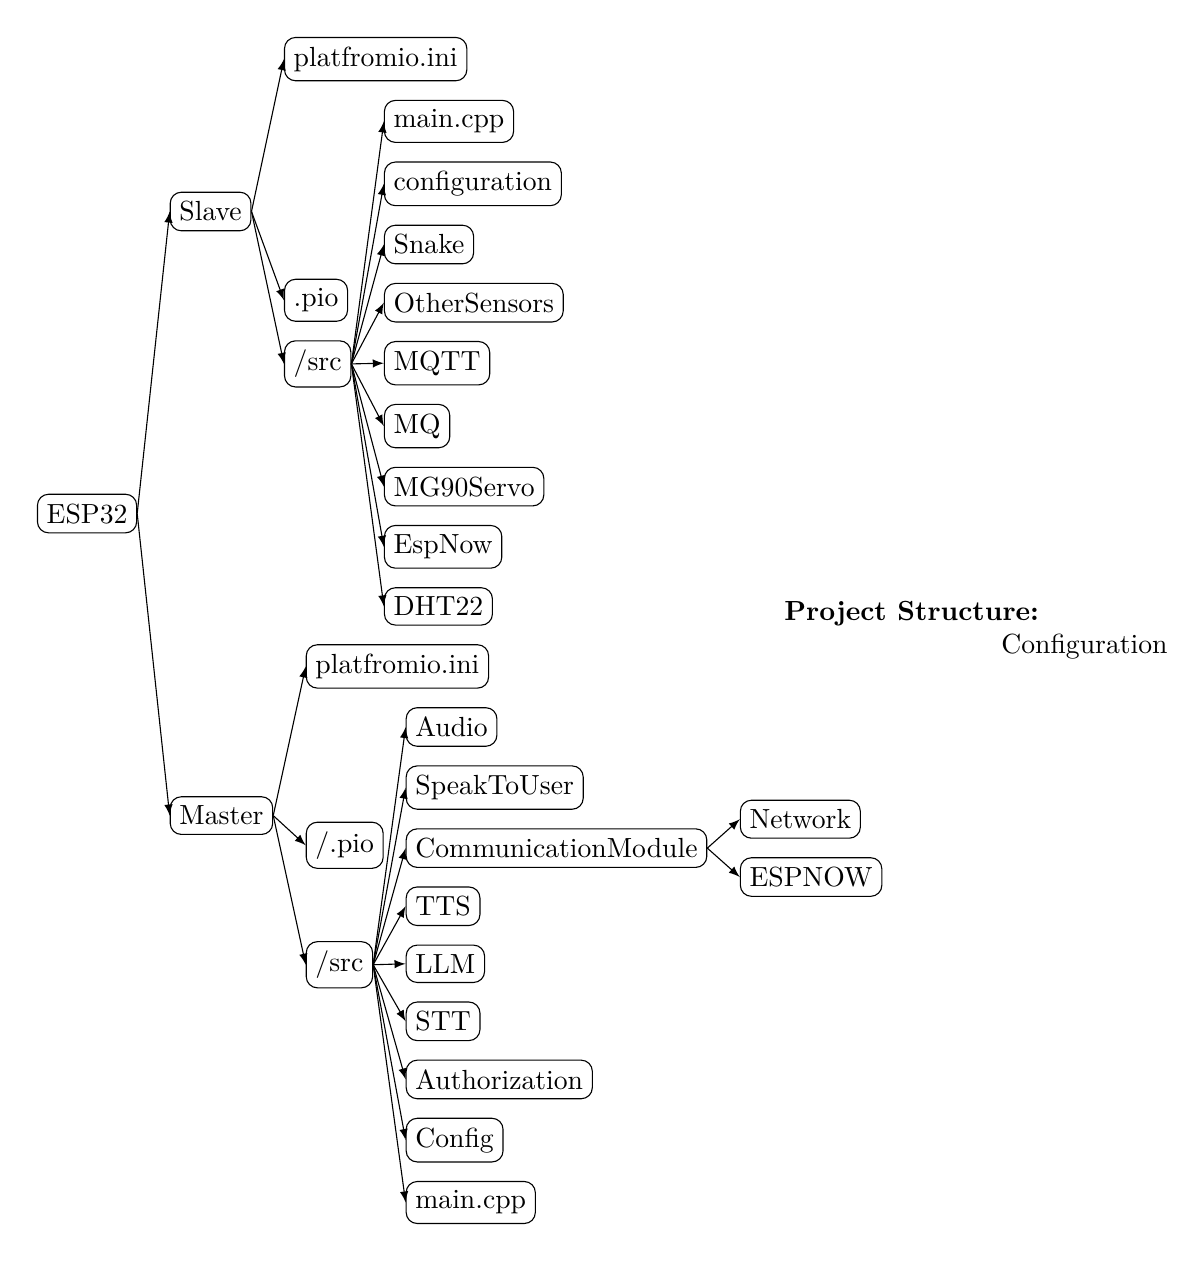
\begin{tikzpicture}
    % 绘制 forest 树结构
    \node at (0, 0) {
        \begin{forest}
            for tree={
                grow=east,
                draw,
                edge={-latex},
                rounded corners,
                node options={align=center},
                anchor=west,
                parent anchor=east,
                child anchor=west,
                delay={where content={}{shape=coordinate}{}},
            }
            [ESP32
                [Master
                    [/src
                        [main.cpp]
                        [Config]
                        [Authorization]
                        [STT]
                        [LLM]
                        [TTS]
                        [CommunicationModule
                            [ESPNOW]
                            [Network]
                        ]
                        [SpeakToUser]
                        [Audio]
                    ]
                    [/.pio]
                    [platfromio.ini]
                ]
                [Slave
                    [/src
                        [DHT22]
                        [EspNow]
                        [MG90Servo]
                        [MQ]
                        [MQTT]
                        [OtherSensors]
                        [Snake]
                        [configuration]
                        [main.cpp]
                    ]
                    [.pio]
                    [platfromio.ini]
                ]
            ]
        \end{forest}
    };

    % 在右侧添加文本
    \node[anchor=west] at (4, 0) { % 调整 x 方向的偏移量以调整文本位置
        \begin{minipage}{0.4\textwidth} % 调整 minipage 的宽度来控制文本框大小
            \textbf{Project Structure:}\\
            项目的树状结构如图所示,最初编译时我将所有的头文件都置于Configuration中,每一份文件都包含它,导致编译非常缓慢,于是将不重合的部分库取出,单独置于需要的文件中,编译速度显著提升。
        \end{minipage}
    };

\end{tikzpicture}

\subsection{参考资料}
\begin{itemize}
    \item Ollama API文档:\href{https://github.com/ollama/ollama/blob/main/docs/api.md\#create-a-model}{\underline{https://github.com/ollama/ollama/blob/main/docs/api.md\#create-a-model}}
    \item 心知天气API文档:\href{https://seniverse.yuque.com/hyper\_data/api\_v3}{\underline{https://seniverse.yuque.com/hyper\_data/api\_v3}}
    \item 讯飞API接口文档:\href{https://xfyun.cn/doc}{\underline{https://xfyun.cn/doc}}
    \item OneNET平台文档:\href{https://open.iot.10086.cn/doc/v5/fuse/detail/920}{\underline{https://open.iot.10086.cn/doc/v5/fuse/detail/920}}
    \item —————————— 参考了很多Github库中的Example —————————————
    \item ESPRessif各种库文档:\href{https://docs.espressif.com/projects/arduino-esp32/en/latest/libraries.html}{\underline{https://docs.espressif.com/projects/arduino-esp32/en/latest/libraries.html}}
    \item U8g2 OLED库:\href{https://github.com/olikraus/u8g2}{\underline{https://github.com/olikraus/u8g2}}
    \item ArduinoJson库:\href{https://arduinojson.org/}{\underline{https://arduinojson.org/}}
    \item HTTPClient库:\href{https://github.com/espressif/arduino-esp32/tree/master/libraries/HTTPClient}{\underline{https://github.com/espressif/arduino-esp32/tree/master/libraries/HTTPClient}}
    \item ESP-I2S协议库:\href{https://github.com/schreibfaul1/ESP32-audioI2S}{\underline{https://github.com/schreibfaul1/ESP32-audioI2S}}
    \item Adafruit开源硬件公司各常用模块、传感器介绍网站:\href{https://lastminuteengineers.com/electronics/arduino-projects/}{\underline{https://lastminuteengineers.com/electronics/arduino-projects/}}
    \item ——————————————————————————————————————————
    \item 【波特律动】在线串口调试助手:\href{https://serial.keysking.com/}{\underline{https://serial.keysking.com/}}
    \item VOFA+ 1.3.10:\href{https://www.vofa.com/}{\underline{https://www.vofa.com/}}
    \item ——————————————————————————————————————————
    \item MPU6050姿态解算2-欧拉角\&旋转矩阵:\href{https://zhuanlan.zhihu.com/p/195683958}{\underline{https://zhuanlan.zhihu.com/p/195683958}}
    \item 学习心得|基于卡尔曼滤波的MPU6050姿态解算:\href{https://www.bilibili.com/video/BV1sL411F7fu}{\underline{https://www.bilibili.com/video/BV1sL411F7fu}}
    \item 对MQ系列传感器采集电压与浓度转换的公式的探索:\href{https://zhuanlan.zhihu.com/p/453499554}{\underline{https://zhuanlan.zhihu.com/p/453499554}}
    \item 南京大学CSI前沿技术分享:\href{https://www.bilibili.com/video/BV1Cv411q7Cz}{\underline{https://www.bilibili.com/video/BV1Cv411q7Cz}}
    \item 新版微信小程序连接到OneNET平台:\href{https://blog.csdn.net/2401\_83704192/article/details/138913230}{https://blog.csdn.net/2401\_83704192/article/details/138913230}
    \item ESP32发声:\href{https://github.com/MetaWu2077/Esp32\_VoiceChat\_LLMs}{https://github.com/MetaWu2077/Esp32\_VoiceChat\_LLMs}
    \item 微信开发者工具使用文档:\href{https://developers.weixin.qq.com/miniprogram/dev/devtools/edit.html}{https://developers.weixin.qq.com/miniprogram/dev/devtools/edit.html}
    \item ——————————————————————————————————————————
    \item Unix时间戳转换工具:\href{https://www.jyshare.com/front-end/852/}{\underline{https://www.jyshare.com/front-end/852/}}
    \item ESPNOW 通信不成功:\href{https://esp32.com/viewtopic.php?p=132946}{\underline{https://esp32.com/viewtopic.php?p=132946}}
    \item ——————————————————————————————————————————
    \item 华东师范大学软件学院实验报告、Beamer模板(本人所作):\href{https://github.com/Shichien/ECNU-LateX-Template}{https://github.com/Shichien/ECNU-LateX-Template}
\end{itemize}

\subsection*{Special Thanks}
 @ Azazo1

 @ Luryem

\end{document}